\documentclass[
	cleardoublepage=plain,
	open=any,
	parskip=half,
]{scrreprt}

\usepackage{amsmath}
\usepackage{amssymb}
\usepackage{mathtools}
\usepackage{unicode-math}

\renewcommand{\frac}[2]{\genfrac{}{}{0.5pt}{0}{#1}{#2}}

\counterwithout{equation}{chapter}

\input{amend/luatex-round-rule-endcaps}
\input{amend/table-of-contents-dotting}

\setkomafont{disposition}{\normalfont}

\RedeclareSectionCommands[toclinefill=\hfill]{section,subsection}

\setcounter{tocdepth}{1}

\usepackage{libertinus}

\usepackage[
	automark,
	autooneside=false,
]{scrlayer-scrpage}

\usepackage[aux]{rerunfilecheck}

\usepackage[american]{babel}

\usepackage[
	backend=biber,
	style=../literature/style,
]{biblatex}
\addbibresource{../literature/books.bib}
\addbibresource{../literature/papers.bib}

\usepackage{xcolor}
\definecolor{RUB}{RGB}{0,53,96}
\definecolor{TUDO}{RGB}{99,154,0}

\usepackage[
	allcolors=RUB,
	citecolor=RUB,
	colorlinks=true,
	english,
	linkcolor=.,
	pdfusetitle,
	pdfcreator={},
	pdfproducer={},
	unicode,
]{hyperref}

\usepackage[
	locale=US,
	per-mode=reciprocal,
	print-unity-mantissa=false,
	print-zero-exponent=true,
	scientific-notation=true,
	separate-uncertainty=true,
]{siunitx}
\DeclareSIUnit\erg{erg}
\DeclareSIUnit\esu{esu}
\DeclareSIUnit\gauss{G}

\usepackage{microtype}


\clearpairofpagestyles

\ihead{\leftmark}
\ohead{\ifstr{\leftmark}{\righttopmark}{}{\righttopmark}}

\cfoot*{\pagemark}

\pagestyle{scrheadings}


\begin{document}

	\begin{titlepage}
		\centering
		\null
		\vspace{9.0\baselineskip}
		{\Huge{Neutrinos via Charm Decays in Astrophysical Sources}\par}
		\vspace{4.5\baselineskip}
		by\par
		{\Large{\textsc{Fritz Ali Agildere}\par}}\href{mailto:fritz.agildere@udo.edu}{fritz.agildere@udo.edu}
		\vfill\null
\end{titlepage}


	\newpage\pagenumbering{gobble}
	
	\null\vfill
	\begin{tabular}{rl}
		First assesment: & P{\kern-0.25pt}.{\kern+0.25pt}D. Dr. Dominik Elsässer \emph{({\kern+0.5pt}Technische Universität Dortmund)} \\
		Second assessment: & Prof. Dr. Julia Tjus \emph{({\kern+0.5pt}Ruhr{\kern+0.5pt}-Universität Bochum{\kern-0.5pt})} \\
		Submission date: & July 25, 2024 \\
	\end{tabular}

	\begin{otherlanguage}{ngerman}
	\chapter*{Zusammenfassung}

	Mit dem Aufkommen der Multimessenger{\kern+0.2pt}-Astronomie zeichnen sich Neutrinos zunehmend als vielversprechende
	Botenteilchen zur Untersuchung hochenergetischer astrophysikalischer Prozesse ab. Bei sehr hohen Energien können Zerfälle
	exotischer Hadronen, die mindestens ein Charm-{\kern+0.3pt}Quark enthalten, aufgrund ihrer kurzen Lebensdauer dominante
	Beiträge zur gesamten Neutrinofluenz liefern. Ziel dieser Arbeit ist die Untersuchung der relativen Signifikanz solcher
	Charmed{\kern+0.1pt}-Hadronen im Kontext verschiedener astrophysikalischer Quellen. Dazu wurden junge und stark
	magnetisierte Neutronensterne sowie die Akkretionsscheiben aktiver Galaxienkerne als Quellregionen modelliert.
	Mit Hilfe analytischer Parametrisierungen und numerischer Integration wurden die so ermittelten Protonenspektren
	dann in Hadronen und schließlich Neutrinos übersetzt. Durch diese semianalytische Rechnung konnte qualitativ gezeigt
	werden, dass es möglich ist Charm-Beiträge zum Neutrinofluss bei hohen Energien zu isolieren. Es wurden
	Probleme mit dem Vorgehen identifiziert, die auf unvollständige Grundannahmen hindeuten. Diese
	sollten weiter untersucht und mit robusteren Methoden korrigiert werden.

\end{otherlanguage}



{\let\clearpage\relax\chapter*{Abstract}\label{ch:abstract}}

With the advent of multimessenger astronomy, neutrinos are increasingly emerging as promising messenger particles for the
study of highly energetic astrophysical processes. At very high energies, decays of exotic hadrons containing at least one
charm quark can represent dominant contributions to the total neutrino fluence due to their short lifetimes. The aim of this
thesis is to investigate the relative significance of such charmed hadrons in the context of different astrophysical sources.
For this purpose, young and strongly magnetized neutron stars as well as the accretion disks of active galactic nuclei were
modeled as source regions. With the aid of analytical parameterizations and numerical integration, the proton spectra obtained
in this way were then translated into hadrons and ultimately neutrinos. This semianalytical calculation qualitatively
demonstrated that it is possible to isolate charm contributions to the neutrino flux at high energies. Problems
with the procedure were identified that point to incomplete basic assumptions. These should be
further investigated and corrected with more robust methods.

	\chapter*{Acknowledgements}
\label{ch:acknowledgements}

I would like to begin by thanking my supervisors, Prof. Dr. Julia Tjus and P{\kern-0.25pt}.{\kern+0.25pt}D. Dr. Dominik Elsässer,
for facilitating the preparation of this thesis and for their review of my work.

Many thanks are also due to Marcel Schroller, who guided me through this complex subject
area, for the interesting discussions and his detailed proofreading of this thesis.

Special thanks also go to David Pape, who took the time to thoroughly check my work
for linguistic correctness and provided me with helpful advice.

Moreover, I wish to express my gratitude to all those who have welcomed and helped me in
both Bochum and Dortmund, of whom there are too many to mention.

Lastly, I want to thank my parents for their continued support, especially my mother,
who has enabled me to concentrate fully on writing this thesis over the last few weeks.

\vfill

I hereby declare that I am the sole author of this thesis and that I have not used
any sources other than those listed in the bibliography and identified as references.
To assist with translation and formulation, the online service \emph{DeepL} was used.
Other tools such as generative artificial intelligence or similar were not employed.

Fritz Agildere\newline{July 24, 2024}


	\chapter*{Abbreviations}
\label{ch:abbreviations}

\begin{description}
	\item[AGN] Active Galactic Nucleus
	\item[CMB] Cosmic Microwave Background
	\item[DSA] Diffusive Shock Acceleration
	\item[FF] Fragmentation Function
	\item[FFE] Force Free Electrodynamics
	\item[GR] General Relativity
	\item[GZK] Greisen-Zatsepin-Kuzmin
	\item[MHD] Magnetohydrodynamics
	\item[QCD] Quantum Chromodynamics
	\item[QED] Quantum Electrodynamics
	\item[QF{\kern+0.5pt}T] Quantum Field Theory
	\item[QM] Quantum Mechanics
	\item[SM] Standard Model
	\item[SMBH] Super{\kern+0.2pt}-Massive Black Hole
	\item[SR] Special Relativity
	\item[UHECR] Ultra-High-Energy Cosmic Ray
\end{description}


	\tableofcontents
	{\renewcommand*{\chaptermarkformat}{}\renewcommand*{\sectionmarkformat}{}\chaptermark{}}
	\enlargethispage{2\baselineskip}\newpage

	\renewcommand{\listfigurename}{Figures}\listoffigures
	{\renewcommand*{\chaptermarkformat}{}\renewcommand*{\sectionmarkformat}{}\chaptermark{}}
	\begingroup
	\let\clearpage\relax
	\renewcommand{\listtablename}{Tables}\listoftables
	{\renewcommand*{\chaptermarkformat}{}\renewcommand*{\sectionmarkformat}{}\chaptermark{}}
	\endgroup

	\newpage\pagenumbering{arabic}

	\chapter{Introduction}
\label{ch:introduction}

	\let\backupskip\chapterheadstartvskip
\renewcommand*\chapterheadstartvskip{\vspace*{3\topskip}} 
\chapter{Background}
\label{ch:background}
\let\chapterheadstartvskip\backupskip

On their journey through space, messenger particles are subject to various influences, both in terms of type and scale,
before reaching our planet. Understanding this propagation requires a thorough comprehension of physical processes at all
scales of application, from production in astrophysical sources, through interactions with the vast radiation and matter
fields that fill the cosmos, to entering the solar system and ultimately the terrestrial atmosphere. The following sections
provide an incomplete overview of aspects relevant to the treatment of this complex topic, as well as references for further
study on the various related subjects.



\section{Particle Physics}
\label{sec:particle}

In our modern view, interactions and categories of elementary particles are most accurately described by a construct called the
\emph{Standard Model} (SM) of particle physics. Underlying this formalism is the mathematical framework known as
\emph{Quantum Field Theory}~(QF{\kern+0.5pt}T{\kern+0.5pt}) that combines and generalizes properties of
\emph{Quantum Mechanics}~(QM) and \emph{Special Relativity}~(SR) to produce a consistent description of microscopic reality.
Excitations in the associated fields are referred to as quanta and manifest themselves as observable particles.
Since this work is mostly concerned with the statistical behaviour of large quantities instead of individual particle probabilistics,
a more detailed treatment is omitted, with the exception of certain phenomena important to the justification of some later assumptions.



\subsection{Fundamental Interactions}
\label{sub:interactions}

With the theory of \emph{Quantum Electrodynamics} (QED) representing a quantized description of classical electromagnetism, the
first successful QF{\kern+0.5pt}T formulation had been realized. It governs all interactions between electrical charges that involve
photons and predicts observations with extremely high precision. Each subsequent QF{\kern+0.5pt}T is built on a foundation of QED
achievements, such as \emph{Quantum Chromodynamics} (QCD) for strong force interactions or the unified framework of
\emph{Electroweak Theory} (EWT) that includes both weak force and electromagnetic phenomena.

According to the SM formalism, these interactions are mediated by bosonic elementary particles, namely massless photons
$\gamma \kern+0.75pt$ for electrodynamics or gluons $\kern-0.5pt g$ in case of the strong force sector, as well as massive
$Z$ and $W^\pm$ bosons that carry the weak force. The only remaining fundamental interaction not contained in the SM is gravity,
the effects of which are currently best described in terms of \emph{General Relativity} (GR{\kern+0.25pt}) as the continuous
macroscopic curvature of spacetime due to the presence of large masses. Because elementary particles exclusively inhabit
microscopic scales, their behavior is usually indistinguishable from that described by SR in flat space.


\subsection{Hadrons \& Leptons}
\label{sub:hadrons}

In addition to the previously listed gauge bosons, the SM further includes elementary fermions as the fundamental constituents of
matter. These sort into the categories of quarks and leptons, both of which are further grouped by generations of quark or lepton
pairs. Ordered according to their generation, there are flavors of up and down, charm and strange, as well as top and bottom for
quarks, which are denoted by their initial letters. For charged leptons, there exist electrons $e$ as well as the heavier muon
$\kern-0.5pt \mu$ and tau $\kern-0.5pt \tau \kern+0.5pt$ that each have an associated neutrino $\nu \kern+0.5pt$ with no electrical
charge. This picture is completed by the corresponding antiquarks and antileptons for all particles mentioned above.

Apart from an electrical charge, quarks are also carriers of so-called color charges that couple to gluons, which, in contrast
to the electrically neutral photons, carry colors themselves. Gluons are therefore capable of self-{\kern+0.25pt}coupling,
leading to higher binding energies with increasing distances. If removed far enough, this energy is eventually
released by producing a quark pair, ultimately leading to the creation of bound color-neutral states.

These resulting composite particles are called hadrons, with the entire process being referred to as hadronization. This naturally
leads to the concept of confinement, which states that quarks cannot exist as free particles, with the notable exception of very
high energies. In these regimes, strong force coupling becomes small and allows quarks to behave almost freely, defining the term
asymptotic freedom. A major consequence of this is that perturbative QCD calculations become possible, which would otherwise
require complex approaches such as discrete QCD on a lattice or some type of effective field theory instead.

The quark model enables classification of hadrons based on their constituent numbers. Baryons are comprised of three quarks, all
with different colors, while mesons contain two quarks with opposite color and anticolor charges. From spin addition, it is clear
that baryons obey fermionic statistics, while mesons act as bosons. Exemplary quark contents are given for baryons such as protons
$p \equiv uud \kern+0.5pt$ and neutrons $n \equiv udd \kern+0.5pt$ as well as pions
$\pi^- \kern-1.0pt \equiv \kern+0.75pt \overline{\kern-0.5pt u \kern+0.5pt} d \kern+0.5pt$ and kaons
$K^- \kern-1.0pt \equiv \kern+0.75pt \overline{\kern-0.5pt u \kern+0.5pt} s \kern+0.5pt$ in the case of mesons.
The charmed hadrons considered in this work are the same mesons
$D^0 \kern-0.75pt \equiv c \kern+1.25pt \overline{\kern-0.5pt u \kern+0.5pt} \kern+0.5pt$ as well as
$D^- \kern-1.0pt \equiv \kern+0.5pt \overline{\kern-0.25pt c \kern+0.75pt} d \kern+0.5pt$
and $D^-_s \kern-1.0pt \equiv \kern+0.5pt \overline{\kern-0.25pt c \kern+0.75pt} s \kern+0.5pt$
with the baryon $\Lambda^{\kern-0.5pt +}_{\kern+0.5pt c} \kern-0.5pt \equiv u \kern+0.5pt d \kern+0.5pt c \kern+0.5pt$
as in \cite{Carpio_2020}. Specific decay channels will be listed directly in the relevant sections
with \cite{pdg} providing a broad overview.

Contrary to hadrons, leptons are fundamental particles. Due to being colorless, they are not affected by the strong force, meaning
that all leptonic interactions obey EWT instead. Noting that photons only couple to electrical charges, this leaves neutrinos as the
only particles which interact exclusively via the weak force. Here, one distinctive feature of the weak interaction should be
mentioned as well, namely that of parity violation. This manifests by only coupling to left-handed components of particles and
right-handed components of antiparticles. Handedness in this context refers to chirality, which for massless particles is equivalent
to helicity or the sign of the spin projection onto the momentum vector. Because the SM assigns zero mass to neutrinos, this EWT
property suppresses certain decay modes and enforces correlated polarizations for the involved leptons. Not included in the SM is
the observation of neutrino oscillations, which are, however, not relevant for this work, since flavor differences are neglected.



\subsection{Reference Frames}
\label{sub:frames}

Depending on the application, energies in particle physics are either given as viewed from a suitable rest frame or independent from
the choice of coordinates altogether. One particularly convenient formulation uses incoming and outgoing momenta
$p_1 , \kern-1.0pt p_2$ and $p_3 \kern+0.5pt , \kern-1.0pt p_4$ to define
\begin{align*}
	s = \bigl( p_1 \kern-0.5pt + p_2 \bigr)^2 &&
	t = \bigl( p_1 \kern-0.5pt - p_3 \bigr)^2 &&
	u = \bigl( p_1 \kern-0.5pt - p_4 \bigr)^2
\end{align*}
as the Mandelstam variables, which assign different channels to scattering processes based on the squared momentum carried by an
exchanged mediating particle. Implied in this context is a Minkowski inner product, making the above quantities manifestly Lorentz
invariant. When working with parametrizations defined for use in different subdisciplines, it regularly becomes necessary to convert
from center of mass energies $\sqrt{s \kern+1.0pt} \kern+1.0pt$ to the energy $\kern-0.5pt E \kern+1.0pt$ of a projectile as viewed
in the system of a stationary target, where vectors $P = (E \kern+1.0pt , \bm{P} \kern+0.75pt c)$ and $p = (m c^2 \kern-1.0pt , 0)$
represent the respective particle momenta. With $\bm{P}$ denoting a classical projectile momentum and $c$ the speed of light,
rest masses $M$ and $m$ for projectile and target lead to a relation $E^2 = \bm{P}^2 c^2 + M^2 c^4$ and
\begin{equation*}
	s = (P + p)^2 = (E + m c^2)^2 - \bm{P}^2 c^2 = 2E m c^2 + \kern+1.0pt m^2 c^4 + M^2 c^4
\end{equation*}
for the invariant mass. The trailing terms in this equation become negligible at high energies, allowing for an approximation
$s = 2E m c^2$ in the target rest frame.



\subsection{Particle Collisions}
\label{sub:collisions}

Another important aspect of particle physics is the description of collision processes. For this purpose, the concept of cross
sections $\sigma \kern+0.5pt$ should be understood. In classical mechanics, these quantities are solely related to geometric
properties of the objects involved, assuming they only interact upon impact. If longer range forces are included, the
cross section represents a larger effective area that measures how the trajectory of an incoming projectile is influenced by
the target. Additionally, differential cross sections with respect to some independent variable such as solid angle
$d\sigma \kern-0.3pt / \kern-0.6pt d\Omega$ or kinetic energy $d\sigma \kern-0.3pt / \kern-0.6pt dE$ can be defined.
Measurements of this quantity often reveal more information about the inner structure of targets. To distinguish these cases,
one might refer to $\sigma$ as the integrated cross section. Since QM is at the core of particle physics, cross sections in this
context are instead interpreted as probability measures of fundamentally stochastic collision processes, such as the production
of specific particles. It can also be useful to separate cross sections into elastic and inelastic components, especially for
collisions in which particles lose energy, as is the case for cooling processes via scattering.



\subsection{Cooling \& Decay}
\label{sub:cooling}

Consider an infinitesimally thin slice of a target medium with particle number density $n$ and volume $V \kern-0.1pt = S \kern+1.5pt dx$
where $S \kern+0.5pt$ and $dx$ measure surface area and thickness, respectively. Accordingly, there exist $\tilde{N} \kern-1.2pt = nV$
targets that each have effective interaction cross sections $\tilde{\sigma}$ with a total coverage of $\tilde{S} = \tilde{\sigma} \tilde{N}$
as viewed by an incident projectile.

The probability for dissipating these beam constituent then corresponds to the ratio $\mathscr{P} = \tilde{S} / S$ of both areas or
explicitly $\mathscr{P} = \kern-0.5pt \tilde{\sigma} \kern+0.5pt n \kern+1.5pt dx$ in case of $dx$ as the covered distance.
Expressing $\tilde{\sigma} = \kappa\sigma$ in terms of the inelastic scattering cross section $\sigma$ and a dimensionless factor
$\kappa$ called inelasticity, one can identify a length scale $\lambda = (\kappa\sigma n)^{-1}$ as the mean free path between
collisions. Multiplying with $\kappa$ includes the ratio of remaining to initital energy, which is taken to be constant. From this
follows a reduction in beam particles $dN \kern+0.1pt = - N \lambda^{-1} dx$ proportional to $N \kern+1.0pt$ as the total projectile
count and $\mathscr{P} = \kern-0.6pt \lambda^{-1} dx$ for the reformulated probability which represents an ordinary differential equation
of first order. The solution is found to follow an exponential law
\begin{equation*}
	N(x) \kern+0.4pt = N_0 \exp \Bigl( -\frac{\raisebox{-0.5ex}{$x$}}{\raisebox{0.5ex}{$\lambda \kern+0.3pt$}} \kern+0.5pt \Bigr)
\end{equation*}
where $N \kern+1.0pt$ particles remain over some distance $x \kern+0.5pt$ with $N_0$ as the initial amount. Furthermore,
\begin{equation*}
	P(x) \kern+0.3pt = 1 -
	\kern+0.9pt \exp \Bigl( -\frac{\raisebox{-0.5ex}{$x$}}{\raisebox{0.5ex}{$\lambda \kern+0.3pt$}}\kern+0.5pt \Bigr)
\end{equation*}
gives the probability of a particle having been scattered after travelling $x \kern+0.5pt$ length units. Similar steps
for time instead of distance lead to the well known equation
\begin{equation*}
	N(t) \kern+0.4pt = N_0 \exp \kern-2.0pt
	\raisebox{0.25ex}{\(\Bigl( \raisebox{-0.25ex}{\(-\frac{\raisebox{-0.5ex}{$t$}}{\raisebox{1.0ex}{$\tau \kern+1.0pt$}}\)}
	\kern+0.5pt \Bigr)\)}
\end{equation*}
describing exponential decay. It commonly appears in the context of radioactive materials but also applies to hadrons and leptons
or more generally any quantity which decreases at a rate proportional to itself. Analogous to the previous case, a particle
decays with probability
\begin{equation*}
	P(t) \kern+0.3pt = 1 - \kern+0.9pt \exp \kern-2.0pt
	\raisebox{0.25ex}{\(\Bigl( \raisebox{-0.25ex}{\(-\frac{\raisebox{-0.5ex}{$t$}}{\raisebox{1.0ex}{$\tau \kern+1.0pt$}}\)}
	\kern+0.5pt \Bigr)\)}
\end{equation*}
before a time $t$ has passed and for $\tau$ as the mean lifetime. Translating this from rest frame to laboratory coordinates defines
the decay timescale $t_\text{dec} \kern-0.6pt = \tau \kern+0.4pt \varGamma$ with a Lorentz factor $\varGamma = E / m$ via
projectile energy and invariant mass. This is equivalent to a characteristic decay length given by
$\lambda_\text{dec} \kern-0.5pt = v \kern+1.5pt t_\text{dec}$ where the velocity $v = c$ can be set for highly relativistic particles.
Additionally, mean free path and cooling distance $\lambda_\text{cool} = (\kappa\sigma n)^{-1}$ refer to exchangeable concepts. Particles
lose energy in every collision, which is the same as reducing temperature from a thermodynamics perspective. Dividing by the speed of
light $c$ translates this expression to $t_\text{cool} = (\kappa\sigma n \kern+0.5pt c)^{-1}$ as a cooling timescale. Analogously, the
distance $\lambda_\text{dec} \kern-0.5pt = c \kern+0.8pt \tau E / m$ can be rewritten as
$t_\text{dec} \kern-0.6pt = \tau E / m$ in units of time. Substituting into the decay formula yields a cooling factor
\begin{equation}
	\mathscr{C} = 1 - \kern+0.9pt \exp \biggl( -\frac{t_\text{cool}}{\raisebox{0.5ex}{$t_\text{dec}$}} \biggr)
	\label{eqn:cooling}
\end{equation}
that rescales spectra from direct production to account for decay processes taking place after collisional energy losses have occured.
This is an essential mechanism for the hypothesis that neutrinos from charm dominate pion and kaon contributions at high energies.
While longer lived particles experience significant cooling thanks to time dilation, charmed hadrons decay promptly in comparison, resulting
in a neutrino flux that directly traces the underlying hadronic spectrum. One requirement for the validity of \eqref{eqn:cooling} is that
$\lambda_\text{dec} \kern-0.3pt \ll d \kern+0.5pt$ holds, with $d \kern+0.5pt$ measuring the target field size to ensure decays occur exclusive
inside this region. 


\newpage\input{amend/special-head}


\section{Multimessenger Astronomy}
\label{sec:multimessenger}

An extension of traditional astronomy, the field of multimessenger astrophysics continues to thrive, providing valuable insights via the
combination of complementary information carried by multiple messenger species. This section begins by expanding on phyiscal concepts
alluded to in chapter \ref{ch:introduction} before continuing to describe the available multimessenger candidates in some detail. For
a more extensive overview, reference \cite{Meszaros_2019} should be consulted.



\subsection{Magnetic Field Scales}
\label{sub:fields}

Particles carrying electric charges $Q = Ze$ and moving at velocity $v \kern+1.0pt$ orthogonal to a homogenous magnetic field $B$ are
acted on by the Lorentz force $F = QvB \kern+0.5pt$ that produces a gyrating motion. With the elementary charge $e$ and $\varGamma$
as a Lorentz factor, this must balance a relativistic centripetal force $F = m \varGamma v^2 \kern-0.5pt / R$ on the resulting circular
path with $R$ giving the Larmor radius. Rearranging and identifying $p = m \varGamma v \kern+0.5pt$ leads to the solution
\begin{equation*}
	R = \frac{p}{\raisebox{0.3ex}{$QB \kern+0.3pt$}}
\end{equation*}
on which the magnetic field extent $D$ imposes $R < D$ as a condition. In case of highly relativistic energies, one can substitute
$E = \kern-0.8pt pc$ for the momentum to obtain an inequality $E < QcBD \kern+0.5pt$ from the above considerations. Realistic astrophyiscal
magnetic fields are not ordered, instead following turbulences that travel through the plasma. To incorporate effects of moving scattering
centers, a factor $\kern-0.5pt \beta \kern+0.5pt$ proportional to the Alfvén velocity is included, giving
\begin{equation}
	E < Ze \kern-0.3pt \beta \kern+0.9pt cBD
	\label{eqn:hillas}
\end{equation}
as the Hillas criterion. It is named after its description in \cite{Hillas_1984} and connects source region sizes to the strength of
prevailing magnetic fields, with observed cosmic ray energies as a constraint.



\subsection{High Energy Cutoff}
\label{sub:cutoff}

At very high energies, protons and nuclei interact with cosmic photons, which can be blueshifted up to extreme gamma regimes due to
the Doppler effect. In these processes, the photon spin is absorbed to produce a delta resonance $\Delta^+$ representing an excited
proton state. This decays almost immediately to pairs of nucleons and pions, leading to $p\gamma \rightarrow \kern-0.1pt n\smash{\pi^+}$
or $p\gamma \rightarrow \kern+0.2pt p \smash{\pi^0}$ as probable reaction channels and resulting in a change of momentum for the
produced particles.~For the case of \emph{Cosmic Microwave Background} (CMB) radiation, a close to perfect black body spectrum
\begin{equation*}
	\frac{\raisebox{-0.3ex}{$dn$}}{\raisebox{0.15ex}{$d\epsilon$}} (\epsilon) \kern+0.2pt =
	\frac{\raisebox{-0.3ex}{$\epsilon^2$}}{\pi^2 \hbar^3 c^3 \bigl( e^{\kern+1.0pt \epsilon / k_B T} - 1 \bigr)}
\end{equation*}
is given by \cite{Gaisser_2016} as the number density. From a CMB temperature of $T \kern-0.5pt = \qty{2.725}{\kelvin}$ follows that
significant photon numbers exist with energies around $\epsilon \kern+0.5pt = \qty{e-12}{\giga\electronvolt}$ in the CMB rest frame. 

\newpage\input{amend/normal-head}

To find a threshold in center of mass coordinates, the scalar product is used for
\begin{equation*}
	s \kern+0.3pt = \bigl( p_{\kern-0.5pt p} + p_{\kern+0.5pt \gamma} \bigr)^2 =
	p_{\kern-0.5pt p}^2 + p_{\kern+0.5pt \gamma}^2 + 2 p_{\kern-0.5pt p} p_{\kern+0.5pt \gamma} =
	m_p^2 \kern+0.8pt c^4 \kern-0.2pt + 2 E \epsilon = \kern-0.2pt M^2c^4
\end{equation*}
where $M \kern-0.3pt = m_p + \kern+0.3pt m_\pi$ and $m_\gamma = 0$ as well as head on collisions have been assumed. The solution
\begin{equation*}
	E = \Bigl( \kern-1.0pt \bigl( m_p + m_\pi \bigr)^2 c^4 \kern-0.2pt - m_p^2 \kern+0.8pt c^4 \Bigr) / (2\epsilon)
\end{equation*}
corresponds to roughly $E \kern+1.0pt = \kern-0.5pt 10^{1 \kern-0.3pt 1} \kern+1.5pt \unit{\giga\electronvolt}$ for the so-called
GZK cutoff. Energies that exceed this value when viewed from \abbrev{CMB} coordinates lead to significant losses, making the universe
opaque to such protons. If pair production $\gamma \kern-0.5pt \rightarrow \smash{e^+ \kern-0.5pt e^-}$ from proton interactions is
considered, one finds
\begin{equation*}
	E = \Bigl( \kern-1.0pt \bigl( m_p + 2m_e \bigr)^2 c^4 \kern-0.2pt - m_p^2 \kern+0.8pt c^4 \Bigr) / (2\epsilon)
\end{equation*}
or approximately $E \kern+1.0pt = \kern-0.5pt \qty{e+9}{\giga\electronvolt}$ by setting $M \kern-0.3pt = m_p + \kern+0.3pt 2m_e$
instead. For alpha particles and heavier nuclei, similar steps apply, while electrons are limited mainly through Compton
downscattering. Additionally, there exist infrared and radio backgrounds as potentially relevant radiation fields. From
the multiple competing mechanisms for energy losses and momentum isotropization, it is as a consequence extremely challenging
to reliably interpret cosmic ray signals and practically impossible to reconstruct any information about specific sources.



\subsection{Stochastic Acceleration}
\label{sub:acceleration}

From the introduction of theoretical limits in sections \ref{sub:fields} and \ref{sub:cutoff} arises the question of how
particles reach these high energy regimes in the first place. Due to its relatively simple derivation and surprising accuracy
in the description of measured spectra, probabilistic collisions are often viewed as one of the most plausible mechanisms
responsible for cosmic ray acceleration. The general case is described in \cite{Longair_2011} and supposes that for each
collision, particles gain some energy proportional to a constant factor $\eta$ and remain in the accelerating region with
probability $\varsigma$ on average. With initial conditions $N_0$ for the number of particles and $E_0$ as the mean
energy, this results in $N \kern+0.9pt = N_0 \varsigma^k$ and $E \kern+0.9pt = E_0 \eta^k$ after $k$ collisions. Using
$\ln x^k = k\ln x$ in
\begin{equation*}
	\frac{\ln (N \kern+1.0pt / N_0)}{\ln (E / E_0)} = \frac{\ln(\varsigma)}{\ln(\eta)}
\end{equation*}
eliminates the exponent and by rearranging gives the relation
\begin{equation*}
	N \kern+0.9pt = N_0 \left( \frac{\raisebox{-0.3ex}{$E$}}{\raisebox{0.3ex}{$E_0$}} \right)^{\ln(\varsigma) / \kern-0.5pt \ln(\eta)}
\end{equation*}
as a connection between energy and particle number. This incidentally follows a power law, which is an almost ubiquitous feature
observed in cosmic ray physics.

\newpage

One can interpret the above expression as an integrated spectrum, leading to
\begin{equation*}
	\frac{\raisebox{-0.3ex}{$dN$}}{\raisebox{0.3ex}{$dE$}} = \frac{\raisebox{-0.3ex}{$N_0$}}{\raisebox{0.3ex}{$E_0$}}
	\left( \frac{\raisebox{-0.3ex}{$E$}}{\raisebox{0.3ex}{$E_0$}} \right)^\alpha
\end{equation*}
for the differential case with a characteristic spectral index
\begin{equation*}
	\alpha = \frac{\ln(\varsigma)}{\ln(\eta)} - 1
\end{equation*}
constrained by $\ln(\varsigma) / \kern-0.5pt \ln(\eta) < 0$ due to $\varsigma < 1$ and $\eta > 1$ as implied per the definitions.

The basic case of \emph{Diffusive Shock Acceleration} (DSA) considers shock fronts that propagate with velocity
$\kern-0.5pt \beta = v / c \kern+1.0pt$ in a fully ionized gas. Requiring momentum isotropization without significant energy losses
on each side of the discontinuity results in $\ln(\varsigma) / \kern-0.5pt \ln(\eta) = -1$ and a corresponding spectral dependence
$dN \kern+0.5pt / dE \propto \kern-0.5pt E^{\kern+0.5pt -2}$ that is discussed by \cite{Longair_2011} as well. A slightly steeper
index around $\alpha = \num{-2.5}$ can be derived when nonlinear effects are accounted for.

Energy gain increasing linearly with $\kern-0.5pt \beta \kern+1.0pt$ leads this mechanism to be categorized as Fermi type acceleration
of first order, whereas the originally proposed formulation scales like $\beta^2$ or as second order. Though shocks exceed the local
speed of sound in the astrophysical medium, relativistic velocities are typically not achieved. Consequently, ratios of $\beta \ll 1$
mean that lower order processes are much more efficient in reaching high particle energies.



\subsection{Cosmic Rays}
\label{sub:rays}

Consisting of charged particles with strictly non-thermal origins, cosmic rays were first detected at high altitudes over a
century ago. Since then, they have become a foundational piece in our understanding of astrophysical sources. Although their flux
is dominanted by protons, other nuclei as heavy as lead can contribute significant portions at high energies as well. Besides this
baryonic component, there are also charged leptons adding to the total population. The exact ratios of these constituents contain
information about source compositions, though any reconstruction of individual sources is likely impossible. This is a result
of cosmic magnetic fields that scramble the directions of charged particles, leading to a largely isotropic distribution. At the
same time, it is possible to constrain the size and field parameters of sources based on the energy of cosmic rays. For this
purpose, section \ref{sub:fields} provides the so-called Hillas condition. In combination with the characteristic broken power
law spectrum, one concludes that most cosmic rays are of galactic origin, except for the highest energies, which require
extragalactic sources \cite{Tjus_2020, Drury_2012}. Beyond these ranges, there appears to be a sharp drop that agrees with
\ref{sub:cutoff} in case of a GZK cutoff. Both the spectral shape and the extreme energies are also consistent with a slightly
modified DSA scenario as described in section \ref{sub:acceleration} for cosmic rays \cite{Becker_2008}.



\subsection{Neutrinos}
\label{sub:neutrinos}

Their weakly interacting nature introduced by section \ref{sub:hadrons} is precisely what makes neutrinos so interesting. After
being produced, they penetrate most obstacles that would be completely opaque to any other messenger particle. This comes at the
cost of being notoriously difficult to detect, of course, but opens up the opportunity of measuring otherwise inaccessible processes
occurring deep inside astrophysical sources. Several different populations are either known or hypothesized, for example
those of solar origin, neutrinos from core-collapse supernovae, steller remnants or active galaxies that are treated in this work,
as well as neutrinos from pion decay implied in section \ref{sub:cutoff} after GZK photodissociation. Additionally, a primordial
neutrino background is expected to exist with a history analogous to that of CMB formation, in which photons decoupled
from matter during the recombination epoch. All of these astrophysical and cosmological prospects as well as the previously
mentioned flavor oscillations make neutrino astronomy a promising field of research.



\subsection{Photons}
\label{sub:photons}

With visual observations being conducted for millenia, photonic signals undoubtedly form the most ancient form of astronomy.
Advances in optical instrumentation have driven revolutionary progress over the last centuries, culminating in modern detectors
unlocking wavelengths across the entire electromagnetic spectrum. Especially radio and gamma frequencies have the potential of
contributing to multimessenger astrophysics, with radio waves having the ability to resolve regions obscured by dust, and gamma
photons being closely associated with hadronic processes in a similar manner as neutrinos, for instance.



\subsection{Gravitational Waves}
\label{sub:gravitational}

Setting aside the possibility of gravitons as hypothetical mediating particles, gravitation seems to be a fundamentally continuous
phenomenon, in the same way as classical theories like that of electromagnetism by Maxwell. According to Einstein, masses lead to
distortions of spacetime that propagate at the speed of light. From this perspective, it readily follows that especially massive
systems such as black hole or neutron star binaries emit gravitational waves through their movement. These excitations have an
advantage compared to other messengers in that they experience essentially no absorbtion or scattering by matter. Alongside unimpeded insights
into highly energetic merger events, there should also exist a gravitational background radiation containing information about
the very early universe.



\section{Astrophysical Sources}
\label{sec:sources}



\subsection{Magnetars}
\label{sub:magnetars}



\subsection{Pulsar Spindown}
\label{sub:spindown}

To explain observations of rapidly spinning neutron stars or pulsars, there has to exist some mechanism by which rotational energy is
lost. Reference \cite{Alvarez_2004} gives a brief overview of possible radiation candidates such as gravitational quadrupolar or
higher order electromagnetic moments. Because this work is limited in its scope and concerns itself with the acceleration of
electric charges, a pure magnetic dipole approach will be adopted. For more compact and convenient notation, Gaussian units are used.

In an idealized view like \cite{Deutsch_1955} of stars as sharply bound and uniformly magnetized spheres, one finds
$\mu = \kern-0.1pt R^3 B / 2$ for the external magnetic moment. The parameters $R$ and $B$ measure stellar radius and polar magnetic
flux density, respectively. In case of a rotating dipole in vacuo,
\begin{equation}
	L = \frac{2\mu^2 \omega^4 \kern-1.0pt \sin^2 \kern-2.0pt \chi \kern+1.0pt}{3c^3}
	\label{eqn:vacuum}
\end{equation}
is the exact expression for radiant power derived in \cite{Jackson_1999} as a standard reference, where a static angle
$\kern-1.0pt \chi \kern+1.0pt$ between the dipole field and rotational axis with angular frequency $\omega$ is assumed. If
instead a \abbrev{FFE} limit is applied, variational calculations \cite{Gruzinov_2006} and \abbrev{MHD} simulations
\cite{Spitkovsky_2006} indicate
\begin{equation}
	L = \frac{\mu^2 \omega^4 \raisebox{0.15ex}{\( \bigl(
	\raisebox{-0.15ex}{\( 1 \kern-0.7pt + \sin^2 \kern-2.0pt \chi \kern+1.0pt \)} \bigr) \)} }{c^3}
	\label{eqn:ffe-mhd}
\end{equation}
as an appropriate expression of the luminosity. This is likely somewhat more accurate than the previous result, as it has been
shown by \cite{Goldreich_1969} that the surroundings of a neutron star cannot support a vacuum but must instead be filled with a
plasma of charge carriers originating from instabilities at the surface. However, one immediately encounters the problem that
$\bm{E} \cdot \kern-1.0pt \bm{B} = \kern-0.5pt 0$ as a condition of force free magnetospheres prevents particle acceleration. As
\cite{Li_2012} and \cite{Gralla_2019} discuss, this can be overcome by introducing deviations from such a global solution on local
scales.

Spindown is described by an exponential energy decay $E = \kern-0.3pt E_0 \kern-0.2pt \exp \kern-2.0pt
\smash{\bigl( - \kern+0.5pt t \kern+0.1pt / \kern+0.2pt t_\text{sd} \kern+0.5pt \bigr)}$ with a characteristic timescale
$t_\text{sd}$ and $\dot{E} = - E / t_\text{sd}$ for the time derivative. Assuming all energy is stored in
rotational form, the expressions $E = \kern-0.5pt I \kern+0.5pt \omega^2 \kern-1.5pt / 2$ and
$\dot{E} = \kern-0.5pt I \kern+0.5pt \omega \kern+0.5pt \dot{\omega}$ are also valid with $I \kern+0.5pt$ as the neutron star
moment of inertia. Equations \eqref{eqn:vacuum} and \eqref{eqn:ffe-mhd} can be generalized as $L = \kern-0.5pt K \omega^4$ by
using a coefficient $K$ containing all other information except the dipolar $\omega^4$ dependence. Identifying this with the energy
loss via $\dot{E} = -L$ and evaluating at $t \kern-0.3pt= 0$ yields $L_0 \kern-0.3pt = \kern-0.2pt K \omega_0^4$ as well as
$\dot{E}_0 \kern-0.3pt = -I \omega_0^2 / 2 \kern+0.4pt t_\text{sd}$ for an expression of
$t_\text{sd} = I \kern+0.5pt / 2K\omega_0^2$ as the spindown time. It further follows for any $t \kern+0.5pt$ that
$I \kern+0.5pt \dot{\omega} = -K \omega^3$ must hold. This is a special case of the power law differential equation
$\dot{\omega} \propto \omega^n$ with $n = 3$ being the braking index characteristic of a rotating magnetic dipole. Separating
variables and integrating leads to finding
$\omega = \omega_0 \smash{\bigl( 1 + \kern+1.5pt t \kern+0.1pt / \kern+0.2pt t_\text{sd} \kern+0.5pt \bigr)^{-1/2}}$
as the time dependent frequency solution.



\subsection{Active Galactic Nuclei}
\label{sub:nuclei}

\cite{Murase_2023} \cite{Visser_2008} \cite{Abramowicz_2013} \cite{Blandford_2019}



\subsection{Accretion Disks}
\label{sub:accretion}

Diffusely distributed material in orbit around a central massive object naturally produces disk like structures. This is a
consequence of gravitational forces being compensated in the radial plane by rotational effects while matter is relatively
free to collapse in the axial direction. 


\newpage\input{amend/normal-head}


Compression and friction during inward spiraling heat the disk, thereby emitting intense thermal radiation. Settings where these
phenomena likely occur are protoplanetary disks surrounding newly formed stars or accretion flows on a \abbrev{SMBH} inside the galactic
core region, among others. The following describes some related effects that are for example discussed by \cite{Longair_2011} as well.



\subsubsection*{Hydrostatic Equilibrium}

In Newtonian physics, the gravitational force at distance $R \kern+0.5pt$ from a mass $M \kern+0.5pt$ is given as
\begin{equation}
	F = \frac{\raisebox{-0.3ex}{$GMm$}}{R^2}
	\label{eqn:newton}
\end{equation}
for particles with masses $m$ orbiting the central object. The resulting acceleration is therefore of magnitude
$g \kern-0.3pt = GM / \smash{R^2}$ with vertical component $\ddot{z} = \kern-0.6pt g \sin(\vartheta)$ and
$\vartheta \kern+0.5pt$ as the angular elevation.~In case of $\kern+0.5pt \vartheta \ll \pi / 2$ one can approximate
$\sin(\vartheta) = \kern+0.3pt z / \kern-0.2pt R \kern+0.5pt$ to obtain
\begin{equation*}
	\ddot{z} = \frac{\raisebox{-0.3ex}{$GMz$}}{R^3}
\end{equation*}
which is related to pressure $p \kern+0.5pt$ and density $\kern-0.5pt \rho \kern+0.5pt$ via
$d \kern-0.1pt p / \kern-0.1pt dz = -\rho \ddot{z} \kern+0.5pt$ for a stable equilibrium to exist. Using the speed
of sound $\smash{u^2} \kern-0.7pt = d \kern-0.1pt p / \kern-0.1pt d \kern-0.1pt \rho \kern+0.5pt$ allows reformulation to
\begin{equation*}
	\frac{d \kern-0.1pt \rho}{\raisebox{0.2ex}{$dz \kern+1.0pt$}} =
	-\rho \kern+1.0pt \frac{\raisebox{-0.3ex}{$GMz$}}{u^2R^3}
\end{equation*}
and $\rho \kern+0.6pt = \kern-0.6pt \rho_0 \kern-0.5pt \exp \kern-1.0pt \smash{\bigl( -z^2 \kern-1.8pt / 2 h^2 \bigr)}$
after integration. According to this result, the disk density follows a centered Gaussian distribution with height parameter
$h \kern+0.5pt$ defined via
\begin{equation*}
	h^2 = \frac{\raisebox{-0.3ex}{$u^2R^3$}}{\raisebox{0.2ex}{$GM \kern+1.5pt$}}
\end{equation*}
as the standard deviation. Assuming $M \gg m$ and circular Keplerian orbits, expression \eqref{eqn:newton} equals the
acting centripetal force, leading to $\smash{v^2} \kern-1.0pt = GM / R \kern+0.2pt$ for the orbital velocity. One is then
able to write $\smash{h^2 \kern-0.5pt = u^2R^2 \kern-1.5pt / v^2}$ and from the necessary condition $h \ll R$ for the small angle
approximation follows $u \ll v \kern+1.0pt$ or that orbital velocities must greatly exceed the speed of sound specific
to the medium. This special case is called a thin disk and can further be extended to slim or even thick types of accretion
structures.



\subsubsection*{Luminosity Limit}

Any luminous object radiating with spherical symmetry excerts a pressure
\begin{equation*}
	P = \frac{\raisebox{-0.3ex}{$L$}}{4\pi R^2 c}
\end{equation*}
as a function of luminosity $L \kern+0.5pt$ at distance $R \kern+0.5pt$ from the source.
Suppose a gaseous cloud containing particles with masses $m$ falling towards the same bright central mass $M \kern+0.5pt$
due to gravitational attraction. During this process, each particle experiences $F = \kern-0.3pt \varkappa \kern+0.7pt mP \kern+0.5pt$
as an opposing radiative force, where the opacity $\kern-0.3pt \varkappa \kern+0.7pt$ measures cross section per unit mass.

\newpage Balancing of \eqref{eqn:newton} and rearranging leads to the Eddington limit
\begin{equation}
	L = \frac{\raisebox{-0.3ex}{$4\pi GM c \kern+0.4pt$}}{\raisebox{0.8ex}{$\varkappa$}}
	\label{eqn:eddington}
\end{equation}
on the luminosity beyond which additional matter is immediately blown away from the central object. By assuming that infalling
material consists exclusively of ionized hydrogen, one can approximate $\varkappa \kern-0.1pt = m / \kern-0.5pt \sigma \kern+0.3pt$
with proton mass $m$ and Thomson cross section $\sigma \kern+0.5pt$ from electron scattering. Though originally applied in the
context of stellar structures, this approach can also be used to describe accretion disks. If a compact object increases its mass
with rate $\dot{M} \kern+0.5pt$ due to accreting matter, some of the corresponding gravitational potential may be converted to
radiation. In terms of rest energy, a luminosity $L = \eta\dot{M}c^2$ is obtained where $\eta$ denotes the efficiency of this
mechanism. With \eqref{eqn:eddington} one finds an analogous steady state limit
\begin{equation*}
	\dot{M} \kern-0.2pt = \frac{\raisebox{-0.3ex}{$4\pi GM$}}{\raisebox{0.8ex}{$\eta c \varkappa$}}
\end{equation*}
for the accretion rate, enforced by continuous balancing of radiation pressure and gravitational forces as a natural feedback process.

	\begin{spacing}{0.975}
	\chapter{Methods}
	\label{ch:methods}
	
	Building on a physical background, this chapter first introduces generally applicable methods for the translation of an
	injected proton distribution to a hadronic spectrum, which then decays to create neutrinos. Subsequently, the injection
	spectra are described for the previously specified astrophysical settings. To start with, a general case $a \rightarrow b$
	is defined for the reaction. Given a spectrum $dN_a \kern+0.5pt / \kern-0.25pt dE_a$ that describes the number $N_a$ of
	particles $a$ per $E_a$ energy interval, as well as the spectral distribution $F_{a \rightarrow b}$ for the probability
	that particles $b$ are produced by a singular interaction, one can obtain their numbers $N_b$ with respect to their
	energies $E_b$ by solving
	\begin{equation}
		\frac{dN_b}{\raisebox{0.5ex}{$dE_b$}} (E_b) \kern+0.5pt = \kern-1.5pt\int_{\check{E}_a}^{\hat{E}_a} dE_a
		\kern+0.5pt \frac{dN_a}{\raisebox{0.5ex}{$dE_a$}} (E_a) \kern+1.5pt F_{a \rightarrow b} (E_b \kern+0.5pt, \kern-0.5pt E_a)
		\label{eqn:folding}
	\end{equation}
	as the corresponding folding integral. From this formulation, it is clear that both distributions and spectra should be assumed
	to depend on energy, with other arguments such as time $t \kern+0.5pt$ being allowed as well. Additionally, it is always necessary
	to specify $\check{E}_a \leq \hat{E}_a$ as integration bounds, which are usually dictated by kinematic constraints.
	
	To implement and compute all following parametrizations, the \emph{Python} programming language and its library \emph{NumPy}
	are used. Graphical results are generated via the \emph{Matplotlib} package.
	
	
	
	\section{Cross Sections}
	\label{sec:cross}
	
	By defining an effective area perpendicular to the momentum vectors of projectiles and targets, cross sections as described
	in Section \ref{sub:collisions} measure probabilities of collision processes in particle physics and are therefore required
	for the calculation of spectral distributions. Distinctions of particle and antiparticle cross sections vanish at high
	energies and are therefore omitted \cite{pdg}.
	
	
	
	\subsection{Scattering}
	\label{sub:scattering}
	
	\enlargethispage*{2\baselineskip}

	To model total cross sections in hadron-proton scattering, this thesis uses the formula
	\begin{equation}
		\sigma_{hp} = H_h \ln^2 \bigl( s \kern+1.0pt / s_h \bigr) + P_h +
		R_h^1 \bigl( s_h \kern+0.5pt / s \bigr)^{\eta_1} + R_h^2 \bigl( s_h \kern+0.5pt / s \bigr)^{\eta_2}
		\label{eqn:hpr1r2}
	\end{equation}
	as given in \cite{Belousov_2016} for a universal analytic parametrization of the corresponding amplitudes.
	All adjustable parameters are listed in Table~\ref{tab:hadron-scattering} together with relevant meson lifetimes for
	cooling. In this approach, the variable $M$ \kern+0.5pt relates to $H \kern+0.5pt = \pi (\hbar c / M)^2$ and
	$s_h \kern-0.5pt = (m_h + m_p + M)^2$ as an effective mass. Coefficients in \eqref{eqn:hpr1r2} are named after Heisenberg,
	Pomeranchuk and Regge, respectively, and have some qualitative motivation, though the formula itself is mainly a quantitative
	result.
	\newpage
\end{spacing}

\begin{table}[H]
	\centering
	\caption[Fits to the total cross sections in hadron proton collisions.]{Fits to the total inclusive scattering cross sections
			 in hadron proton collisions. Parameters are taken from \cite{Belousov_2016} with $M = \qty{2.121}{\giga\electronvolt}$
			 for $H = \qty{0.272}{\milli\barn}$ as the rate of growth. Both $\eta_1 = \num{0.447}$ and $\eta_2 = \num{0.5486}$ are
			 dimensionless exponents. Rest masses $m_h$ can be found in the particle listings \cite{pdg} and are given in natural units.}
	\label{tab:hadron-scattering}
	\sisetup{group-digits=integer, table-format=2.2}
	\begin{tabular}{c S S S[table-format=1.3] S[table-format=1.3] S}
		\midrule\midrule
		{$h$} & {$P_h \mathbin{/} \unit{\milli\barn}$} &
		{$R_h^1  \mathbin{/} \unit{\milli\barn}$} & {$R_h^2  \mathbin{/} \unit{\milli\barn}$} &
		{$m_h \mathbin{/} \unit{\giga\electronvolt}$} & {$s_h \mathbin{/} \unit{\giga\electronvolt\squared}$} \\
		\midrule
		{$p$} & 34.41 & 13.07 & 7.39 & 0.938 & 15.98 \\
		{$\pi$} & 18.75 & 9.56 & 1.767 & 0.140 & 10.23 \\
		{$K$} & 16.36 & 4.29 & 3.408 & 0.494 & 12.62 \\
		\midrule\midrule
	\end{tabular}
\end{table}


Assuming a quasi universal ratio $\mathscr{R}$ between elastic and total hadron cross sections, one obtains the inelastic
cross section $\sigma_\text{inel} = (1 - \mathscr{R}) \sigma_\text{tot}$ from $\sigma_\text{el} = \mathscr{R} \sigma_\text{tot}$
and $\sigma_\text{el} + \sigma_\text{inel} = \sigma_\text{tot}$ as a unitarity condition. Provided in \cite{Fagundes_2012} is
the model-independent parametrization
\begin{equation}
	\mathscr{R}(s) = \frac{\sigma_{\text{el}\kern+0.5pt} (s)}{\sigma_{\text{tot}\kern+0.5pt} (s)} =
	\mathscr{A} \tanh \bigl( \kern+1.0pt \gamma_1 \kern-1.0pt - \gamma_2 \ln (s) + \gamma_3 \ln^2 (s) \bigr)
	\label{eqn:ratio}
\end{equation}
with a constant asymptote $\mathscr{A}$ at very high energies. Coefficients are given in Table \ref{tab:hadron-ratio} for
different physical settings. Both equations \eqref{eqn:hpr1r2} and \eqref{eqn:ratio} use units of \unit{\giga\electronvolt\squared}
for the $s$  variables. Combining these, Figure \ref{fig:hadron-proton-scattering} depicts the scaling of inelastic cross sections
with energy for different hadrons.

\begin{table}[H]
	\centering
	\vspace{2.0ex}
	\caption[Model independent ratio of elastic and total $\sigma_{h \kern-0.1pt p}$ cross sections.]
			{Almost model independent ratio of hadronic elastic
			 and total scattering cross sections. Factors $\gamma$ are taken from \cite{Fagundes_2012} for varying
			 $\mathscr{A}$ asymptotes.}
	\label{tab:hadron-ratio}
	\sisetup{group-digits=integer, table-format=1.4}
	\begin{tabular}{c S S S[table-format=1.5]}
		\midrule\midrule
		{$\mathscr{A}$} & {$\gamma_1$} & {$\gamma_2$} & {$\gamma_3$} \\
		\midrule
		{$1/2$} & 0.466 & 0.0259 & 0.00177 \\
		{$1$} & 0.2204 & 0.0111 & 0.00076 \\
		\midrule\midrule
	\end{tabular}
\end{table}


Reference \cite{Fagundes_2013} examines the asymptotic rise $\sigma(s) \propto \ln^2(s)$ derived in \cite{Froissart_1961}
as a theoretical upper bound and concludes that it is somewhat exceeded. Additionally, an asymptote $\mathscr{A} = 1/3$ due to
diffraction as opposed to the black disk limit $\mathscr{A} = 1/2 \kern+0.2pt$ from optical theorem predictions is suggested
in \cite{Fagundes_2013}. As parameters are only available in the latter case, all calculations of $\mathscr{R}$
use a ratio \eqref{eqn:ratio} as defined by $\mathscr{A} = 1/2 \kern+0.2pt$ for this thesis. Data matching $\mathscr{A} = 1/3$
imply that $\sigma_{\text{inel}\kern+0.5pt}(s)$ is slightly underestimated, though this is unlikely to
noticeably impact the overall results.

\begin{figure}[H]
	\centering
	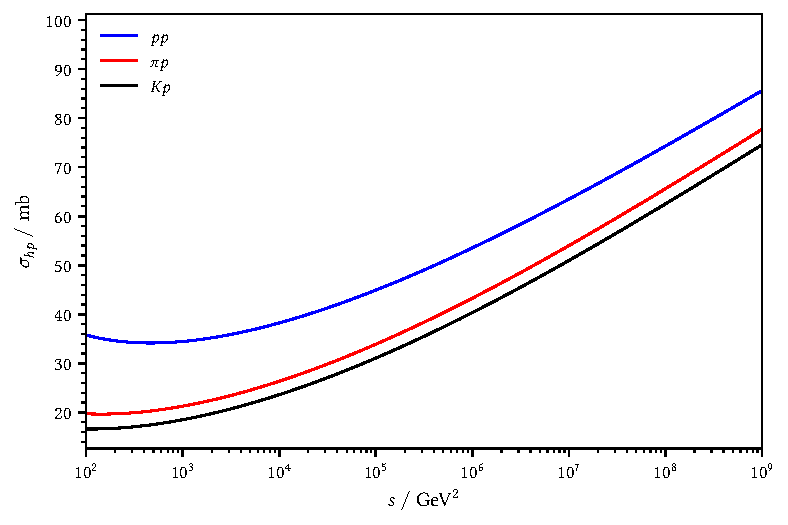
\includegraphics{../plots/build/hadron_proton_scattering.pdf}
	\caption[Inelastic cross sections $\sigma_{h \kern-0.1pt p}$ for hadron-{\kern+0.1pt}proton scattering.]
			{Inelastic cross sections $\sigma_{h \kern-0.1pt p}$ for hadron-{\kern+0.1pt}proton scattering according to the
			 parametrizations \eqref{eqn:hpr1r2} and \eqref{eqn:ratio} reproducing an asymptotic $\cramped{ln^2(s)}$ scaling.}
	\label{fig:hadron-proton-scattering}
\end{figure}




\subsection{Production}
\label{sub:production}

For charm quark production in proton-{\kern+0.1pt}air collisions, reference \cite{Goncalves_2007} gives
\begin{equation}
	x_F \kern+1.0pt \frac{\raisebox{-0.5ex}{$d\sigma$}}{\raisebox{0.5ex}{$dx_F$}} \bigl( x_F \kern+0.5pt, \kern-0.5pt E_p \bigr)
	\kern-0.1pt = a \kern+0.5pt x_F^b \kern+1.0pt \bigl( 1 \kern-0.3pt - x_F^m \kern+0.3pt \bigr)^n
	\label{eqn:charm}
\end{equation}
as the parametrized differential cross section with components
\begin{align*}
	&& a = a_1 \kern-0.5pt \ln\bigl(E_p\bigr) - \kern+0.5pt a_2 \: , && b = b_1 \kern-1.0pt - b_2 \ln\bigl(E_p\bigr) \: , &&
	n = n_1 \kern-1.0pt - \kern+0.5pt n_2 \ln\bigl(E_p\bigr) &&
\end{align*}
for which Table \ref{tab:charm-production} lists all necessary constants. Here, proton energies $E_p$ are defined as viewed
by air nuclei at rest, while the Feynman scaling variable $x_F \kern+1.0pt = p_c \kern+1.5pt / \kern-0.5pt p_s$ specifies
the magnitude ratio of produced charm quark longitudinal momentum to all available momentum in center mass coordinates of the
colliding particles. Application of Section \ref{sub:frames} shows that this approximately fulfills $x_F \kern+1.0pt = x_c$
where $\cramped{x_c = \kern+0.2pt E_c \kern+1.0pt / E_p}$ in the relevant energy ranges. It should be noted that for the values
Table \ref{tab:charm-production} provides, the factor $n_0 \kern-0.5pt = \num{0.075}$ from Table 1 in \cite{Goncalves_2007} 
for the lower energy regime is set to $n_0 \kern-0.5pt = \num{7.5}$ instead, because the parametrization breaks down otherwise.
Further testing reveals another problem with the \qty{e4}{\giga\electronvolt} to \qty{e8}{\giga\electronvolt} region
in that energies of~\qty{26}{\tera\electronvolt}~or lower yield negative differential cross
sections. Considering other approximations made in this thesis, it is therefore decided that an extrapolation from the
\qty{e8}{\giga\electronvolt} to $10^{1 \kern-0.3pt 1} \kern+1.5pt \unit{\giga\electronvolt}$ case to all energies
can be done without producing unreasonably large errors. With these parameters, equation~\eqref{eqn:charm}~only becomes
negative for energies of \qty{140}{\giga\electronvolt} and below.

\begin{table}[H]
	\centering
	\vspace{1.5ex}
	\caption[Parametrization of the $c$ quark differential cross section.]
			{Parametrization of the weighted charm quark
			 production differential cross section. Coefficients are calculated from \cite{Goncalves_2007} to write $E_p$
			 in units of \unit{\giga\electronvolt} without needing redundant conversion steps. The exponent $m = \kern-0.5pt \num{1.2}$
			 is a constant at all energies. For the application at hand, energy ranges beyond the given validity intervals
			 are used as mentioned in the text.}
	\label{tab:charm-production}
	\sisetup{group-digits=integer, table-format=1.3}
	\begin{tabular}{l S[table-format=3.0] S[table-format=4.0] S S S S}
		\midrule\midrule
		{$E_p \mathbin{/} \unit{\giga\electronvolt}$} & {$a_1 \mathbin{/} \unit{\micro\barn}$} &
		{$a_2  \mathbin{/} \unit{\micro\barn}$} & {$b_1$} & {$b_2$} & {$n_1$} & {$n_2$} \\
		\midrule
		{$10^4 - 10^8$} & 826 & 8411 & 0.197 & 0.016 & 8.486 & 0.107 \\
		{$10^8 - 10^{1 \kern-0.3pt 1}$} & 403 & 2002 & 0.237 & 0.023 & 7.639 & 0.102 \\
		\midrule\midrule
	\end{tabular}
\end{table}


Adopting linear scaling with respect to the nucleon number from \cite{Bhattacharya_2015} gives
\begin{equation*}
	\frac{\raisebox{-0.5ex}{$d\sigma$}}{\raisebox{0.5ex}{$dx_c$}} \bigl( x_c \kern+0.5pt, \kern-0.5pt E_p \bigr) = \tilde{A}^{-1}
	\frac{\raisebox{-0.5ex}{$d\sigma$}}{\raisebox{0.5ex}{$dx_F$}} \bigl( x_c \kern+0.5pt, \kern-0.5pt E_p \bigr)
\end{equation*}
for inclusive charm production in proton-{\kern+0.1pt}proton collisions. Approximating air as a gas mixture of roughly \qty{75}{\percent}
nitrogen and \qty{25}{\percent} oxygen, one finds $A = \kern-0.3pt \num{14.5}$ for this factor. By integrating the charmed hadron
cross section defined below and comparing to experimental data in \cite{lhc} for the charm mesons considered in this thesis,
one finds that calculated values exceed measurements~by a factor \num{22.32+-2.34} on average, yielding $\tilde{A} = \num{323.64}$
as a modification to enforce compatibility with observations. One problem of this approach is that \cite{lhc} provides values
at $\sqrt{s \kern+1.0pt} \kern+1.0pt = \qty{13}{\tera\electronvolt}$ or roughly $E_p = \kern+0.1pt \qty{90}{\peta\electronvolt}$ only,
so that deviations at different energies are not accounted for. Similar to earlier reasoning, the resulting inaccuracy is deemed acceptable.

Translation of charm quarks to charmed hadrons is achieved with an integral
\begin{equation}
	\frac{\raisebox{-0.5ex}{$d \kern+1.2pt \tilde{\sigma}$}}{\raisebox{0.5ex}{$dx_h$}}
	\bigl( x_h \kern+0.5pt, \kern-0.5pt E_p \bigr) = \kern-1.0pt \int_{\kern+0.5pt x_h}^1 dz \, z^{-1}
	\frac{\raisebox{-0.5ex}{$d\sigma$}}{\raisebox{0.5ex}{$dx_c$}}
	\bigl( x_c \kern+0.5pt, \kern-0.5pt E_p \bigr) \kern+1.0pt D^{\kern+0.5pt h}_c (z)
	\label{eqn:unmodified}
\end{equation}
where $z = E_h \kern+1.0pt / E_c \kern+0.5pt$ and $x_h = E_h \kern+1.0pt / E_p \kern+0.5pt$ as well as
$x_c = x_h \kern+1.0pt / z$ are fractional energies. Limits for the integration follow from a basic inequality
$E_h \leq E_c \kern+0.2pt \leq E_p$ to incorporate kinematic constraints. Furthermore, the probability
of observing any final state $h$ originating from a $c$ quark is encoded in a \emph{Frag$\kern-0.3pt$mentation Function}
(FF) $D^{\kern+0.5pt h}_c (z)$ dependent on the fraction of hadron to charm energy. Reference
\cite{Metz_2016} addresses the connection between this concept and that of a \emph{Parton Distribution Function}
(PDF) among other things. While a PDF represents the probability density of finding a parton with given momentum inside
a colorless particle, probabilities for color-neutral states existing in individual partons are given by the appropriate
FF instead. The partons described here are either quarks or gluons, which Sections \ref{sub:interactions} and \ref{sub:hadrons}
characterize in more detail.

\newpage

By fitting to existing data or perturbative calculations, models can extrapolate to low momentum fractions that have
not yet been probed experimentally. Such a method has lead \cite{Kniehl_2006} to obtain
\begin{equation}
	D^{\kern+0.5pt h}_{c}(z) = \frac{N_h z \kern+1.0pt (1 - z)^{\kern+0.5pt 2}}
	{\bigl((1 - z)^{\kern+0.5pt 2} + \epsilon_h z \bigl)^{\raisebox{-1.5ex}{$^2$}}}
	\label{eqn:fragmentation}
\end{equation}
with parameters from $\kern+0.5pt e^+e^- \kern-0.8pt$ data in Table \ref{tab:charm-hadrons} as the charm hadron FF used
throughout this thesis. It is important to note that such functions are invariant under charge conjugation, so that there is no
differentiation between quark to particle or antiquark to antiparticle processes.

% \begin{figure}[H]
% 	\centering
% 	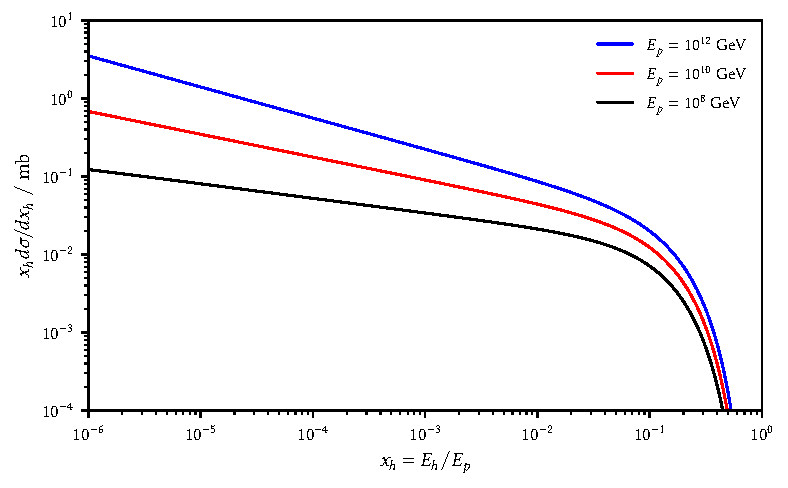
\includegraphics{../plots/build/charm_hadron_cross_section.pdf}
% 	\caption[Inclusive differential cross sections for $\smash{p \kern-0.1pt p \kern+0.6pt \rightarrow D^0 X \kern+0.5pt}$ production.]
% 			{Inclusive differential cross sections for $\smash{p \kern-0.1pt p \kern+0.6pt \rightarrow D^0 X \kern+0.5pt}$ production at
% 			 different proton energies $E_p$ according to the \eqref{eqn:differential} parametrization.}
% 	\label{fig:charm-hadron-cross-section}
% \end{figure}


To account for kinematic constraints, one final modifier has to be included at this point. Because collisions must provide
enough energy for particle formation, charmed hadron energies cannot be lower than their rest masses, leading to
$E_h \geq \kern+0.4pt m_h$ as a natural condition. With Table \ref{tab:charm-hadrons} listing these mass parameters,
a cutoff similar to that in \cite{Kelner_2006} is introduced, rewriting \eqref{eqn:unmodified} to
\begin{equation}
	\frac{\raisebox{-0.5ex}{$d\sigma$}}{\raisebox{0.5ex}{$dx_h$}}
	\bigl( x_h \kern+0.5pt, \kern-0.5pt E_p \bigr) =
	\frac{\raisebox{-0.5ex}{$d \kern+1.2pt \tilde{\sigma}$}}{\raisebox{0.5ex}{$dx_h$}}
	\bigl( x_h \kern+0.5pt, \kern-0.5pt E_p \bigr) 
	\left( 1 - \kern+0.3pt \frac{m_h}{\raisebox{1pt}{$x_h \kern+0.2pt E_p$}} \right)^{\kern-1.0pt 1/2}
	\label{eqn:differential}
\end{equation}
where $E_h \kern-0.3pt = x_h \kern+0.2pt E_p$ ensures physical kinematics are respected. It turns out that this expression
is integrable, whereas the unmodified version \eqref{eqn:differential} is not. Figure \ref{fig:charm-hadron-cross-section}
depicts the $\smash{\cramped{D^0}}$ differential cross section for different incident proton energies and fixed protons as targets.
Comparing this to Figure 7 in \cite{Carpio_2020} indicates similar shapes, though our parametrizations result in less flat
distributions at low $x_h$ values.

\newpage\input{amend/special-head}

\section{Spectral Distributions}
\label{sec:spectral}

Constructing spectra $dN_h \kern+0.5pt / dE_h$ from proton injection requires folding of $F_{p \kern+0.8pt \rightarrow h}$ as
the hadronic distribution for a single $p \kern-0.1pt p \kern+0.9pt$ interaction with the number of protons per energy interval
given by the function $dN_p \kern+0.6pt / dE_p$ obtained from source{\kern+0.1pt}-specific modeling. An analogous approach can
be applied to compute neutrino spectra $dN_\nu \kern+0.6pt / dE_\nu$ from $dN_h \kern+0.5pt / dE_h$ via distributions
$F_{\kern+1.0pt h \kern+0.2pt \rightarrow \nu}$ formulated according to the involved decay modes. Equation \eqref{eqn:folding}
describes exactly this, with the following section providing all required distributions.



\subsection{Charm}
\label{sub:charm}

Spectral distributions for charmed hadron production are calculated according to \cite{Carpio_2020} through
\begin{equation*}
	F_{p \kern+0.8pt \rightarrow h} \bigl( E_h \kern+0.5pt , \kern-0.5pt E_p \bigr) =
	E_p^{\kern+0.5pt -1} \sigma_{p \kern-0.1pt p}^{-1} \bigl( E_p \bigr) \kern+1.0pt
	\frac{\raisebox{-0.5ex}{$d\sigma$}}{\raisebox{0.5ex}{$dx_h$}} \bigl( x_h \kern+0.5pt, \kern-0.5pt E_p \bigr) \: ,
\end{equation*}
with $E_h \kern-0.2pt = x_h E_p$ translating between variables. This can be understood as effectively normalizing term
\eqref{eqn:differential} with respect to the energies and inelastic cross sections of protons, which are scattered as described in
Section \ref{sub:scattering} to yield hadron numbers per unit energy and collision.

To find neutrino spectra from charmed hadrons, the same approach as in \cite{Bhattacharya_2016} is used, which assumes an
effective energy distribution approximated by three{\kern+0.3pt}-body decays for the semileptonic channel to a less massive
pseudoscalar meson. By neglecting lepton masses, one obtains
\begin{equation*}
	\tilde{F}_{\kern+1.0pt h \kern+0.2pt \rightarrow \nu \kern+1.0pt} (y) = D_h^{-1} \kern+1.0pt \Bigl( 6b_ha_h^2 - 4a_h^3
	- 12\lambda_h^2 a_h + 12\lambda_h^2 y - 6b_h y^2 + 4 y^3 + 12 \lambda_h^2 \ln \bigl((1 - y) / \lambda_h \bigr) \Bigr)
\end{equation*}
as a distribution with $y = E_\nu \kern+0.6pt / E_h$ and $F_{\kern+1.0pt h \kern+0.2pt \rightarrow \nu \kern+1.0pt}
\bigl( E_\nu \kern+1.0pt , \kern-0.5pt E_h \bigr) = \mathscr{F}_h \tilde{F}_{\kern+1.0pt h \kern+0.2pt \rightarrow \nu \kern+1.0pt}
(y) / E_h$ for conversion.

Hadron specific coefficients for this equation are defined with the parameter
$\lambda_h = \kern+0.5pt \tilde{s}_h / m_h^2 \kern+0.2pt$ as
\begin{align*}
	a_h = 1 - \lambda_h \: , && b_h = 1 - 2\lambda_h \: , &&
	D_h = 1 - 8 \lambda_h - 12\lambda_h^2 \ln \bigl( \lambda_h \bigr) + 8 \lambda_h^3 - \lambda_h^4
\end{align*}
where both $s_h$ and $m_h$ are listed in Table \ref{tab:charm-hadrons} for all included charmed hadrons. The assumption of
three{\kern+0.3pt}-body decays like $D^+ \kern-2.5pt \rightarrow \kern+1.0pt \overline{\kern-1.5pt K \kern+1.0pt}\kern+1.0pt^0 e^+ \nu_e$
can be justified by consulting \cite{pdg} for information on the relevant particles and comparing branching ratios, which indicate
that purely leptonic modes are strongly suppressed. Hadronic channels such as $D^+ \kern-2.5pt \rightarrow \pi^+ \pi^0$ or
$D^+ \kern-2.5pt \rightarrow K^{\kern+0.5pt -} \pi^+ \pi^+$ are either very improbable as well or occur at significant rates but
do not contribute many high-{\kern+0.2pt}energy neutrinos due to pions and kaons being subject to further cooling before decaying
to leptons. By a similar logic, secondary muon decay is neglected when determining the neutrino spectrum, as muons would experience
additional cooling before decaying and charm cross sections are already low compared to other mesons.

\newpage\input{amend/normal-head}

\begin{spacing}{0.970}
	\begin{table}[H]
	\centering
	\vspace{2.0ex}
	\caption[Coefficients for $c$ hadron production, cooling and decay.]
			{Coefficients for charm hadron production,
			 cooling and decay to neutrinos. All parameters $\epsilon_h$ are taken from leading order QCD fits
			 via the FF as defined and described in \cite{Kniehl_2006} with normalizations $N_h$ given by \cite{Carpio_2020}
			 to rescale the integration of \eqref{eqn:fragmentation} over $[0 \kern+0.5pt , \kern-1.5pt 1]$ to approximately match
			 the fractions $f_h$ provided in \cite{Lisovyi_2016} from measurements. Effective masses $\sqrt{\tilde{s}_h}$ and branching
			 fractions $\mathscr{F}_h$ are determined by \cite{Bugaev_1998} and \cite{Bhattacharya_2016} from fitting decay rates.
			 Mean lifetimes $\tau_h$ and masses $m_h$ are adopted from \cite{pdg} in the particle listings. Mass type
			 quantities use natural units.}
	\label{tab:charm-hadrons}
	\sisetup{group-digits=integer, table-format=1.2}
	\begin{tabular}{c S[table-format=1.4] S[table-format=1.5] S[table-format=4.0] S[table-format=1.3] S S}
		\midrule\midrule
		{$h$} & {$N_h$} & {$\epsilon_h$} & {$\tau_h \mathbin{/} \unit{\femto\second}$} & {$\mathscr{F}_h$} &
		{$\sqrt{\tilde{s}_h} \mathbin{/} \unit{\giga\electronvolt}$} & {$m_h \mathbin{/} \unit{\giga\electronvolt}$} \\
		\midrule
		{$D^{0}$} & 0.577 & 0.101 & 410 & 0.067 & 0.67 & 1.86 \\
		{$D^{+}$} & 0.238 & 0.104 & 1033 & 0.176 & 0.63 & 1.87 \\
		{$D^{+}_{s}$} & 0.0327 & 0.0322 & 501 & 0.065 & 0.84 & 1.97 \\
		{$\Lambda^{\kern-0.5pt +}_{\kern+0.5pt c}$} & 0.0067 & 0.00418 & 203 & 0.045 & 1.27 & 2.29 \\
		\midrule\midrule
	\end{tabular}
\end{table}


	\subsection{Pions \& Kaons}
	\label{sub:pions}
	
	By parametrizing {\textsc{sibyll}}\footnote{
	{\kern+1.5pt}The authors of \cite{Kelner_2006} do not specify the \textsc{sibyll} version that is used.}
	\cite{Fletcher_1994} results, a neutral pion production spectrum of the form
	\begin{equation*}
		\tilde{F}_{p \kern+0.5pt \rightarrow \pi} \kern+1.5pt \bigl( x_\pi \kern+0.7pt , \kern-0.5pt E_p \bigr) = 4\alpha B x_\pi^{\alpha - 1}
		\left( \frac{1 - \kern+0.2pt x_\pi^\alpha}{1 + \kern+0.8pt rx_\pi^\alpha (1 - \kern+0.2pt x_\pi^\alpha \kern+1.0pt )}
		\right)^{\kern-1.0pt 4} \left( ( 1 - \kern+0.2pt x_\pi^\alpha \kern+1.0pt )^{-1} +
		\frac{r (1 - \kern+0.2pt 2x_\pi^\alpha \kern+1.0pt )}{1 + \kern+0.8pt rx_\pi^\alpha (1 - \kern+0.2pt x_\pi^\alpha \kern+1.0pt )}
		\right) \left( 1 - \kern+0.3pt \frac{m_\pi}{\raisebox{1pt}{$x_\pi \kern+1.0pt E_p$}} \right)^{\kern-1.0pt 1/2}
		\label{eqn:pions}
	\end{equation*}
	is found in \cite{Kelner_2006} with $m_\pi = \qty{0.135}{\giga\electronvolt}$ \cite{pdg} translated to natural units and parameters
	\begin{align*}
		&&&& B \kern+0.5pt = \tilde{B} + C \: , &&
		\alpha \kern+0.5pt = \frac{\raisebox{-1.5pt}{$\tilde{\alpha}$}}{\displaystyle\sqrt{C \kern+1.5pt}} \: , &&
		r \kern+1.0pt = \frac{\raisebox{-1.5pt}{$\tilde{r}$}}{\displaystyle\sqrt{C \kern+1.5pt}} &&&&
	\end{align*}
	where a low energy cutoff is enforced via $E_\pi \kern-0.1pt = x_\pi \kern+1.0pt E_p$ in the mass term. From
	\begin{equation*}
		C = c_1 \kern-0.5pt - \kern+0.5pt c_2 \ln \bigl( E_p \bigr) + \kern+0.5pt  c_3 \ln^2 \bigl( E_p \bigr)
	\end{equation*}
	results a dependence on projectile energy for the shape of this distribution.
	
	Coefficients are specified in Table \ref{tab:pion-spectrum} and recalculated from $E_p \kern+0.5pt$ in \unit{\tera\electronvolt}
	to units of \unit{\giga\electronvolt} instead. Under the assumption of a $\smash{\pi^0} \kern-0.5pt$ cross section approximately
	equal to the $\smash{\pi^\pm} \kern-0.5pt$ average and with identical spectra between charged pions, it follows that
	$F_{p \kern+0.5pt \rightarrow \pi} = \tilde{F}_{p \kern+0.5pt \rightarrow \pi} \kern+1.0pt / E_p$ should describe pion
	production regardless of charge reasonably well for the purpose of this thesis.
	
	\enlargethispage*{2\baselineskip}
	\begin{table}[H]
	\centering
	\vspace{2.0ex}
	\caption[Parametrized spectral distribution for pion production.]{Parametrized spectral distribution for
			 neutral pion production. Factors are taken from \cite{Kelner_2006} and converted to write $E_p$
			 in units of \unit{\giga\electronvolt} for $c_k$ coefficients.}
	\label{tab:pion-spectrum}
	\sisetup{group-digits=integer, table-format=1.3}
	\begin{tabular}{S[table-format=1.2] S[table-format=1.2] S[table-format=1.1] S S S}
		\midrule\midrule
		{$\tilde{B}$} & {$\tilde{\alpha}$} & {$\tilde{r}$} & {$c_1$} & {$c_2$} & {$c_3$} \\
		\midrule
		0.25 & 0.98 & 2.6 & 1.515 & 0.206 & 0.075 \\
		\midrule\midrule
	\end{tabular}
\end{table}

	\newpage
\end{spacing}

\begin{spacing}{0.980}
	For a convenient formulation of kaon production, references \cite{Lykasov_2021} and \cite{Lykasov_2022} indicate a constant ratio
	$\pi / K$ at moderately high energies. Similar fractions are retrieved from multiplicities given in \cite{Koers_2006} and lead to
	$F_K \kern+0.5pt / F_\pi = \num{0.12}$ as a simplifying assumption, the validity of which cannot be guaranteed for the application
	at hand. Calculations of kaon spectra still employ this approach but are subject to considerable reservations as a result, because
	fixed ratios to pion spectra are unlikely to be universal. Other than this factor, the pion mass is replaced with that of kaons for
	a correct cutoff in the above expression.
	
	Decays of pions and kaons to neutrinos are approximated via the $h \rightarrow \mu^+ \nu_\mu$ two{\kern+0.2pt}-body channel
	with branching fractions of $\mathscr{F}_{\kern-0.2pt \pi \kern+0.2pt} = \qty{99.99}{\percent}$ and
	$\mathscr{F}_{\kern+0.3pt K \kern+0.2pt} = \qty{63.56}{\percent}$ given in the \cite{pdg}
	particle listings. By decaying, muons produced in these processes can significantly impact the neutrino spectrum. Results from
	\cite{Carpio_2020} suggest that this is particularly relevant for pions. Muonic three{\kern+0.3pt}-body decays of type
	$\mu^- \kern-2.5pt \kern+0.5pt \rightarrow e^- \kern+0.5pt \overline{\kern-0.2pt \nu \kern+0.8pt}_e \nu_\mu$ as well as
	cooling factors depend on the polarization of participating leptons due to the nature of weak force coupling. This complicates
	computations and is thus omitted for the purpose of restricting the present thesis to a manageable scope, though it should be
	remembered as an important caveat for the final results.
	
	The remaining two{\kern+0.2pt}-body decays of ultra-relativistic hadrons $h$ to leptons $l \kern+1.0pt$ obey a distribution
	\begin{equation*}
		F_{\kern+1.0pt h \kern+0.2pt \rightarrow l \kern+1.0pt} \bigl( E_l \kern+0.8pt, \kern-0.2pt E_h \bigr) =
		\mathscr{F}_{\kern+0.2pt h \kern+0.2pt} E_h^{\kern+1.0pt -1} \bigl( 1 \kern-0.3pt - \lambda_h \bigr)^{-1}
	\end{equation*}
	with $m_{\kern+0.5pt \nu} = 0$ and $m_\mu = \qty{0.106}{\giga\electronvolt}$ \cite{pdg} as well as
	$\lambda_h \kern-0.3pt = m_\mu^2 \kern+0.5pt / m_h^2$ as a parameter. This formula is the same whether
	$l = \nu \kern+0.2pt$ or $l = \kern-0.3pt \mu$ because there is one muon for each neutrino. In addition,
	kinematic considerations lead to $E_\mu \kern+0.5pt / E_h > \lambda_h$ and
	$E_{\kern+0.5pt \nu} \kern+0.5pt / E_h < 1 - \lambda_h$ for bounds
	$E_\mu < E_h < E_\mu \kern+0.5pt / \lambda_h$ in case of muons or corresponding limits
	$E_{\kern+0.5pt \nu} \kern+0.5pt / \smash{\bigl( 1 - \lambda_h \bigr)} < E_h < E_p$ when considering neutrinos, which are
	required by \eqref{eqn:folding} for integration.
	
	
	
	\section{Computation}
	\label{sec:computation}
	
	Taking into account previous deliberations, this section now combines these with the contents of Chapter \ref{ch:background}
	to give explicit steps for calculating the results as well as numerical values for the required parameters.
	Additionally, some notes on the implementation are included.
	
	
	\subsection{Injection}
	\label{sub:injection}
	
	The proton spectrum model of young magnetars described in Section \ref{sub:magnetars} starts with an idealized charge density
	$\rho = \omega B_\text{ns} \kern+0.2pt / (2\pi c)$ derived from \cite{Goldreich_1969} and leads to $n = \kern-0.6pt \rho / \kern-0.2pt e$
	for the number of charge carriers. Integrating over the so-called polar caps defined by a radius
	$\smash{R_\text{pc} \kern-1.0pt = \kern-0.2pt R_\text{ns} \sqrt{R_\text{ns} / R_\text{lc}}}$ from which open field lines
	originate and taking a monochromatic energy according to \eqref{eqn:mono} for all times $t \kern+0.5pt$ results
	in a time-derivative delta-functional spectrum
	\begin{equation}
		\frac{d\kern+0.75pt\dot{N}_p}{\raisebox{0.5ex}{$dE_p$}} \bigl( t, E_p \bigr) =
		\frac{B_\text{ns} R_\text{ns}^3 \omega_0^2}{ec \bigl( 1 + \kern+1.5pt t \kern+0.1pt / \kern+0.2pt t_\text{sd} \kern+0.5pt \bigr)}
		\kern+1.0pt \delta \kern+0.5pt \bigl( E_p - E^M(t) \bigr)
		\label{eqn:delta}
	\end{equation}
	that is compatible with a $dN_p \kern+0.5pt / dE_p \propto E_p^{\kern+0.3pt -1}$ power law.
	\enlargethispage*{\baselineskip}\newpage
\end{spacing}

For the AGN setting, a more general DSA scenario like in Section \ref{sub:acceleration} is assumed, yielding
\begin{equation*}
	\frac{dN_p}{\raisebox{0.5ex}{$dE_p$}} \bigl( E_p \bigr) = \mathscr{S} E_p^{\kern+0.2pt -2}
\end{equation*}
with $\kern-0.2pt \mathscr{S} \kern+0.6pt$ for an arbitrary normalization factor that does not need to be specified further,
as this thesis is interested in relative neutrino contributions instead of absolute predictions.



\subsection{Production \& Decay}
\label{sub:decay}

Spectra of hadrons and neutrinos are generally computed as in \eqref{eqn:folding} via folding, though for the hadronic spectrum,
a cooling factor \eqref{eqn:cooling} and optical depth \eqref{eqn:optical} are included, giving
\begin{equation*}
	\frac{dN_h}{\raisebox{0.5ex}{$dE_h$}} \bigl( E_h \bigr) = \mathscr{CO} \int_{E_h}^{\mathscr{E}_{\kern-0.5pt p}}
	\kern-0.5pt dE_p \frac{dN_p}{\raisebox{0.5ex}{$dE_p$}} \bigl( E_p \bigr) \kern+1.5pt
	F_{p \kern+0.8pt \rightarrow h} \bigl( E_h \kern+0.5pt , \kern-0.5pt E_p \bigr)
\end{equation*}
with maximum proton energies $\mathscr{E}_{\kern-0.5pt p}$ as a result. Because the proton spectrum \eqref{eqn:delta}
contains a delta function $\smash{\delta \kern+0.5pt \bigl( E_p - E^M \kern+0.5pt \bigr)}$ in the magnetar case, integration
over $E_p$ simply substitutes $\smash{E^M}$ in place of the proton energy. Accordingly, a limit $\mathscr{E}_{\kern-0.5pt p} = \infty$
can be set to ensure $\smash{E^M} < \mathscr{E}_{\kern-0.5pt p}$ at all times. For the AGN accretion disk, a choice of
$\mathscr{E}_{\kern-0.5pt p} = \smash{\qty{e12}{\giga\electronvolt}}$ is made in accordance with the maximum magnetar proton energy.
A value exceeding that of the GZK cutoff at $E_p = \smash{10^{1 \kern-0.3pt 1}} \kern+1.5pt \unit{\giga\electronvolt}$ described in
Section \ref{sub:cutoff} can be justified by assuming close proximity to the origin of accelerated particles. Proceeding from this,
cross sections and distributions are taken from Sections \ref{sec:cross} and \ref{sec:spectral} to translate the produced hadrons
to neutrinos, which due to their weak interactions mentioned in Section \ref{sub:hadrons} are assumed to be unaffected
by attenuation.

Cooling factors \eqref{eqn:cooling} vary for different hadrons, as $t_\text{dec} \kern-0.5pt = \tau_h E_h / m_h$ and
$t_\text{cool} \kern-0.5pt = \cramped{(\kappa_{h \kern-0.1pt p} \sigma_{h \kern-0.1pt p} n c)^{-1}}$ define the decay and cooling timescales,
with parameters $\tau_h$ and $m_h$ listed in the respective tables, as well as \eqref{eqn:hpr1r2} and \eqref{eqn:ratio} giving the
$\sigma_{h \kern-0.1pt p}$ cross sections, which are approximated to those of kaons for charmed hadrons. The effective optical depth
\eqref{eqn:optical} only describes proton interactions, where the mean free path
$\lambda_{p \kern-0.1pt p} = \cramped{(\kappa_{p \kern-0.1pt p} \sigma_{p \kern-0.1pt p} n)^{-1}}$ and distance $d$ are determined by the
model. Inelasticity factors are assumed to be constants with $\kappa_{h \kern-0.1pt p} = \num{0.8}$ and $\kappa_{p \kern-0.1pt p} = \num{0.5}$
as given in \cite{Carpio_2020}. For the scenario of a newborn magnetar, ejecta properties result in
$n = n_\text{ej}$ \eqref{eqn:number-density} and $d \kern+0.1pt = r_\text{ej}$ \eqref{eqn:ejecta-radius} as parameters. The AGN
accretion disk is modeled by the height parameter \eqref{eqn:height} that varies with radius and characterizes a diffuse density
distribution, as well as the angle $\alpha$ measuring the direction of incidence relative to the disk plane. This is further
simplified by assuming a sharply bound region of height $h$ with homogenous density, leading to $d = h / \kern-2.0pt \sin \alpha$
as the distance travelled by a particle. Because results are insensitive to variations in distance, one can set
$\alpha = \pi \kern+0.25pt / 2$ to find $\sin\alpha = \kern-0.1pt 1$ and $d = h$ with $h = \kern-0.5pt \smash{\qty{e15}{\centi\meter}}$
as stated in \cite{King_2008}. Typical number densities of the order \qty{e15}{\per\centi\meter\cubed} in the disk plane
\cite{Garcia_2013, Garcia_2014} are scaled down to account for the inhomogeneous distribution \eqref{eqn:density} and assumed to be
$n = \kern-0.5pt \smash{\qty{e14}{\per\centi\meter\cubed}}$ for the following calculations. To put this into perspective, typical
SMBH masses of around \qty{e8}{\solarmass} correspond to a \qty{e13}{\centi\meter} Schwarzschild radius. While the radii of accretion disks
can extend to \qty{e18}{\centi\meter} or more, relativistic jets can reach multiple \qty{100}{\kilo\parsec} with terminal bow shocks at
\unit{\mega\parsec} distances from the core \cite{Blandford_2019, King_2008, Murase_2023}.

\newpage

Parameters for the magnetar setting are adopted from \cite{Carpio_2020}. Neutron star radii $R_\text{ns} = \qty{e6}{\centi\meter}$
and masses $M_\text{ns} = \qty{1.4}{\solarmass}$ in accordance with the Chandrasekhar limit that defines the maximum stable mass for
white dwarfs lead to $I_\text{ns} = \qty{e45}{\gram\centi\meter\squared}$ as the classical moment of inertia for a rigid homogenous
sphere, where relativistic effects are ignored and $\qty{1}{\solarmass} = \qty{2e33}{\gram}$ is used. Reference \cite{Haensel_1999}
provides the minimum period of uniform rotation, beyond which the neutron star loses its structural integrity. Choosing twice this
value yields $\omega_0 = \qty{e4}{\per\second}$~as~an~optimistic initial angular frequency. The tilt parameter $\chi$ is set to an
angle of $\chi = \num{0.95}$ radians.~A~magnetic~field of~$B_\text{ns} \kern-0.75pt = \qty{3.2e14}{\gauss}$ leads to a maximum energy
$E^M = \num{5.3} \times 10^{1 \kern-0.3pt 1} \kern+1.5pt \unit{\giga\electronvolt}$ for proton acceleration as well as
$t_\text{sd} = \qty{3.2e3}{\second}$ as the spindown time. With the total ejected mass being similar to that of the
respective progenitor star, values between \qty{10}{\solarmass} and \qty{35}{\solarmass} are possible, from which
the lower bound $M_\text{ej} = \qty{10}{\solarmass}$ is chosen for this scenario. At velocity $\beta_\text{ej} = \num{0.1}$
of the shell, number densities $n_\text{ej} = \smash{\qty{3.1e18}{\per\centi\meter\cubed}}$ are  observed after $t_\text{sd}$
has passed. Lastly, an efficiency $\eta = \num{0.1}$ is assumed for the acceleration of protons.



\subsection{Implementation}
\label{sub:implementation}

In order to calculate neutrino spectra from hadronic distributions, several integrals have to be computed. Discretizing
this computation allows the general case
\begin{align*}
	F(x, y) \kern+1.5pt &= \int_{z_{-}}^{z_{+}} dz \: G(x, z) \, H(z, y) \\
	\intertext{to be rewritten as a Riemann sum. Assuming $G$ and $H$ are integrable over a given interval,}
	F_{ij} \kern+1.8pt &= \sum\nolimits_k D_{kk} \, G_{ik} \, H_{kj}
\end{align*}
converges to the exact solution for sufficiently small subintervals. Transforming variables
\begin{align*}
	&&&& x \rightarrow x_i \: , && y \rightarrow y_j \: , && z \rightarrow z_k &&&&
\end{align*}
and defining $D_{kk} = z_{k+1} \kern-1.0pt - z_k$ leads to the above notation. It is easily shown how this expression in terms of
indices translates to the product of corresponding matrices
\begin{equation*}
	\bm{F} \kern+0.6pt = \bm{G} \, \bm{D} \, \bm{H}
\end{equation*}
as an equivalent formulation. Here, the output $\bm{F} \in \mathbb{R}^{m \times n}$ is obtained from the inputs
$\bm{G} \in \mathbb{R}^{m \times l}$ as well as $\bm{H} \in \mathbb{R}^{l \times n}$ with the square matrix
$\bm{D} \in \mathbb{R}^{l \times l}$ that encodes all step sizes on its diagonal. These results enable a quick and
efficient implementation of the required calculations as program code, where arithmetic array operations can greatly
increase execution speed. Furthermore, logarithmic spacing of $\bm{D}$ often leads to better accuracy after fewer
iterations. To avoid redundant computations, results are stored as data tables.\footnote{
{\kern+1.5pt}For the purpose of reproducibility, all implementations are collected in a dedicated \emph{GitHub} repository:\\
\href{https://github.com/fritzali/bachelor}{github.com/fritzali/bachelor}}



\newpage
\begin{spacing}{0.985}
	\subsection{Event Generation}
	\label{sub:generators}
	
	The description of multiple colliding particle systems constitutes an extremely complex problem, which methods like perturbative
	QF{\kern+0.5pt}T or lattice QCD mentioned in Sections \ref{sub:interactions} and \ref{sub:hadrons} are unable to resolve
	with satisfactory accuracy. Modeling of collider or air shower experiments therefore requires a different approach, realized
	by so-called event generators that fit data in well-tested regions and extrapolate to higher energies via random sampling.
	The Monte Carlo event generator \textsc{sibyll} used as well by \cite{Carpio_2020} and \cite{Kelner_2006} is optimized for
	the simulation of high energy cosmic ray cascades, making it a suitable choice for the calculation of cross sections in an
	astrophysical context such as that of this thesis \cite{Fletcher_1994}.
	
	\begin{figure}[H]
	\centering
	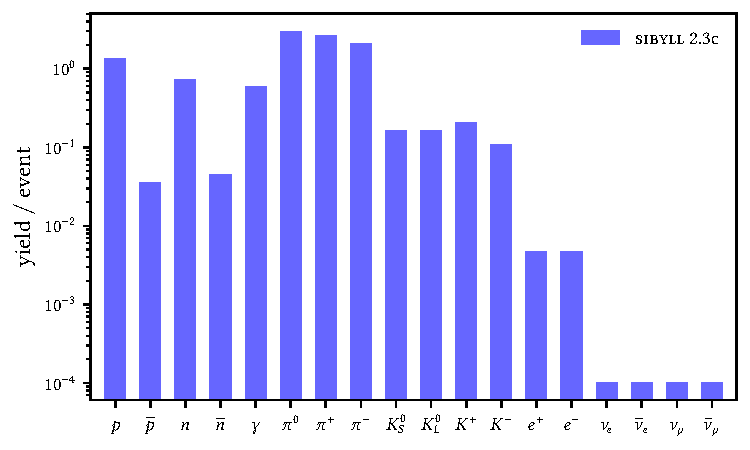
\includegraphics{../plots/build/event_generator.pdf}
	\caption[]
			{}
	\label{fig:event-generator}
\end{figure}

	
	Depicted in Figure \ref{fig:event-generator} are the yields of select particle types per proton-{\kern+0.1pt}proton collision as predicted
	by \textsc{sibyll} 2.3c at $\smash{\sqrt{s \kern+1.0pt} \kern+1.0pt = \qty{1}{\tera\electronvolt}}$ energies. Other particles are
	produced but deemed irrelevant for modeling charm as well as pion and kaon production. This represents one step in the process
	of generating numerical values for the appropriate cross sections. Events are generated at discrete fixed target or center of mass
	energies, with individual yield populations additionally following a separate energy distribution. Accordingly, each bar in
	Figure \ref{fig:event-generator} is an effective integral over all energies of the produced particles. Weighted energy
	differential cross sections $d\sigma \kern+0.5pt / \kern-0.1pt dx$ for specific secondary types can therefore be expressed by a
	histogram in two dimensions, with initial proton energies on one axis and energy of secondaries on the other. Normalizations are
	found by counting the yield and comparing to known values. Creating energy bins at the required resolutions and with sufficient statistics
	is computationally intensive and consumes more time than is available for work on this thesis, which instead uses parametrizations
	as described in the previous sections. Event generator predictions should nevertheless be considered to verify and improve upon the
	following results.
	\enlargethispage*{\baselineskip}\newpage
\end{spacing}

	\chapter{Results}
\label{ch:results}

\begin{figure}[H]
	\centering
	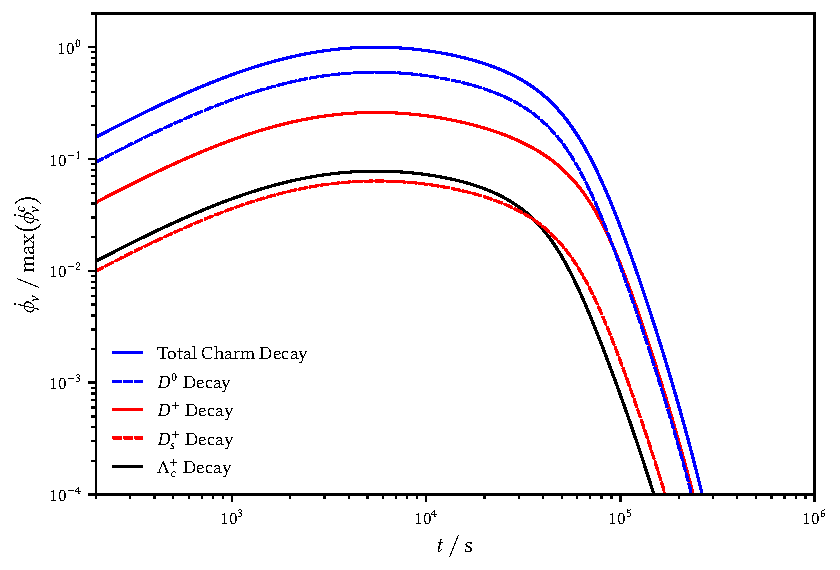
\includegraphics{../plots/build/magnetar_charm_decay_comparison_with.pdf}
	\caption[Magnetar $\nu \kern+0.5pt$ flux from $c$ decay including optical depth.]
			{Comparison of individual charmed hadron contributions to the total charm neutrino flux at
			 $E_\nu = \kern-0.5pt \qty{e9}{\giga\electronvolt}$ from a young magnetar, including the optical
			 depth defined by \eqref{eqn:optical} as a modification. Decays of $\smash{D^0}$ produce most of
			 the charmed neutrinos until later times when $\smash{D^+} \kern-0.5pt$ becomes significant, with
			 $\smash{D^+_s}$ and $\smash{\Lambda^{\kern-0.5pt +}_{\kern+0.5pt c}}$ being similar, both
			 contributing around \qty{10}{\percent} to the combined flux. This is in line with the
			 cross sections from \ref{sub:charm} as well as the branching fractions that
			 Table \ref{tab:charm-hadrons} lists.}
	\label{fig:magnetar-charm-comparison-with}
\end{figure}

\begin{figure}[H]
	\centering
	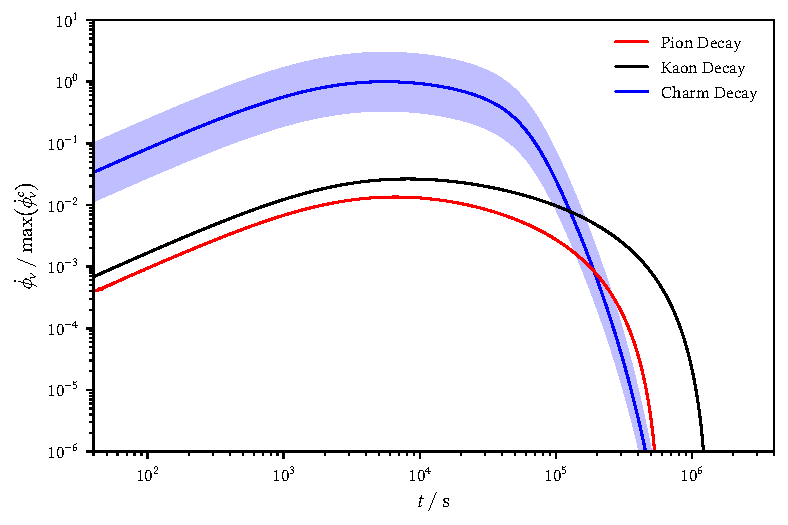
\includegraphics{../plots/build/magnetar_neutrino_spectrum_with.pdf}
	\caption[]{}
	\label{fig:magnetar-flux-with}
\end{figure}

\begin{figure}[H]
	\centering
	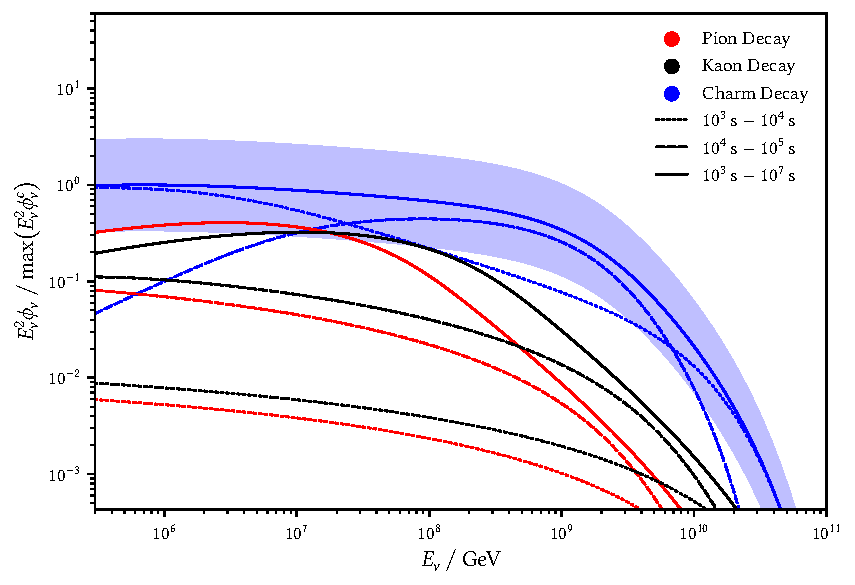
\includegraphics{../plots/build/magnetar_integrated_neutrino_spectrum_with.pdf}
	\caption[Magnetar $\nu \kern+0.5pt$ fluence compared to $c$ decay with optical depth.]
			{Expected neutrino fluence normalized to the maximum charm contribution from a~young magnetar for different time
			 intervals after formation, including the optical depth defined by \eqref{eqn:optical} as a modification.
			 Charmed hadrons dominate at all energies~except below $E_\nu = \kern-0.5pt \qty{e7}{\giga\electronvolt}$ for the
			 $\qty{e4}{\second} - \kern-1.0pt \qty{e5}{\second}$ integration. This is unexpected and therefore discussed further
			 in the text. The same shaded uncertainty band as in Figure \ref{fig:magnetar-flux-with} is adopted for charm decays.
			 Fluences are scaled by a factor $E_\nu^2$ for clarity and to facilitate the comparison to \cite{Carpio_2020}.}
	\label{fig:magnetar-fluence-with}
\end{figure}


\begin{figure}[H]
	\centering
	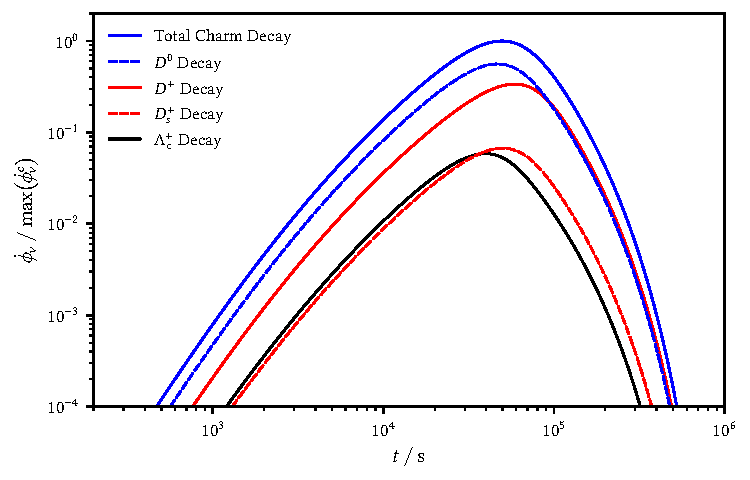
\includegraphics{../plots/build/magnetar_charm_decay_comparison_without.pdf}
	\caption[Magnetar $\nu \kern+0.5pt$ flux from $c$ decay excluding optical depth.]
			{Comparison of individual charmed hadron contributions to the total charm neutrino flux at
			 $E_\nu = \qty{e9}{\giga\electronvolt}$ from a newborn magnetar, excluding optical depth.}
	\label{fig:magnetar-charm-comparison-without}
\end{figure}

\begin{figure}[H]
	\centering
	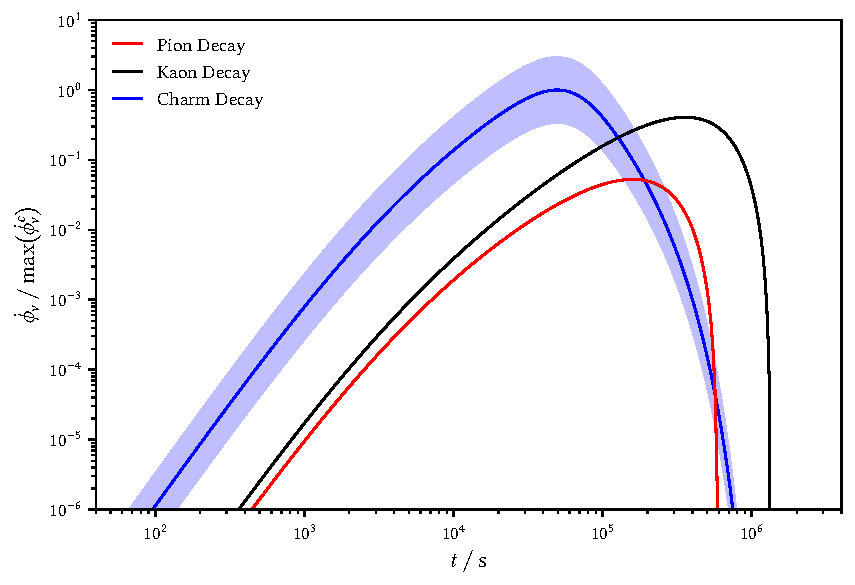
\includegraphics{../plots/build/magnetar_neutrino_spectrum_without.pdf}
	\caption[Magnetar $\nu \kern+0.5pt$ flux compared to $c$ decay without optical depth.]
			{}
	\label{fig:magnetar-flux-without}
\end{figure}

\begin{figure}[H]
	\centering
	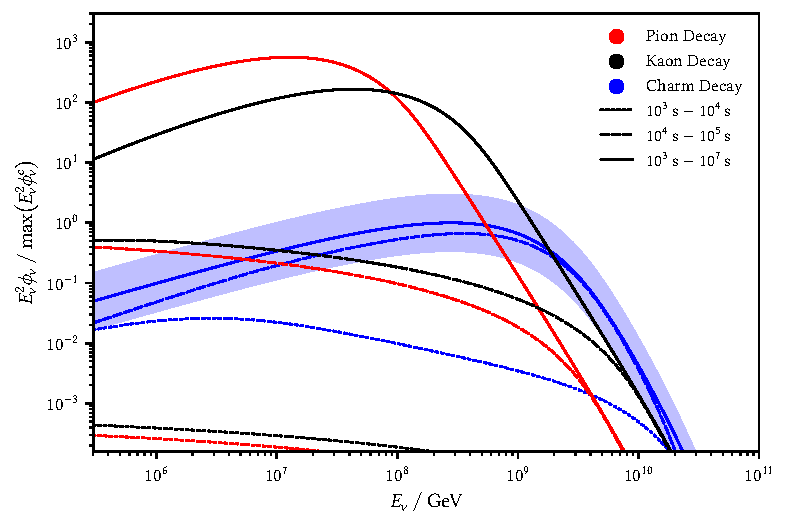
\includegraphics{../plots/build/magnetar_integrated_neutrino_spectrum_without.pdf}
	\caption[]{}
	\label{fig:magnetar-fluence-without}
\end{figure}


\begin{figure}[H]
	\centering
	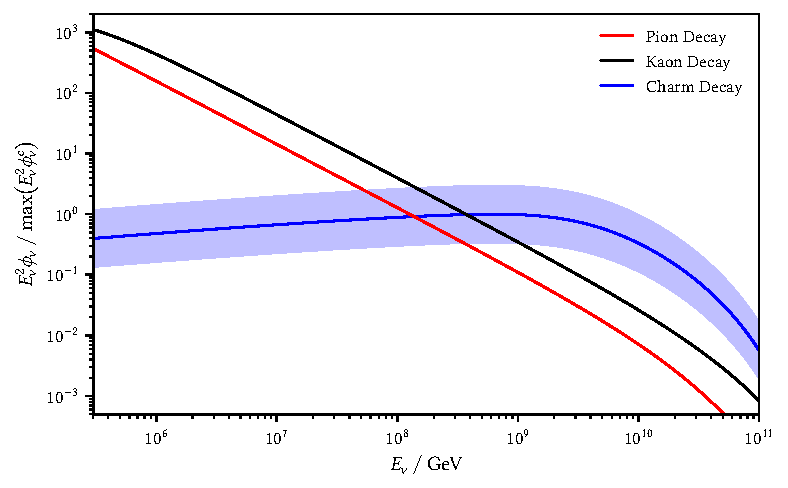
\includegraphics{../plots/build/nucleus_neutrino_spectrum.pdf}
	\caption[AGN accretion disk $\nu \kern+0.5pt$ fluence compared to $c$ decay.]
			{}
	\label{fig:nucleus-fluence}
\end{figure}

\begin{figure}[H]
	\centering
	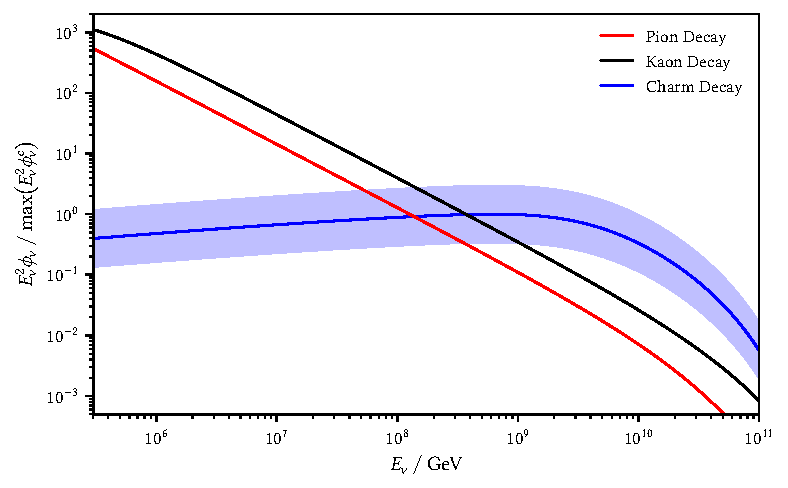
\includegraphics{../plots/build/nucleus_neutrino_spectrum.pdf}
	\caption[AGN accretion disk $\nu \kern+0.5pt$ fluence compared to $c$ decay.]
			{Expected neutrino fluence normalized to the maximum charmed hadron contribution from an AGN accretion disk.
			 Differences between the shapes of pion and kaon components compared to charm decays result from the chosen
			 view, as the flat increase observed for charmed hadrons occurs at lower energies in the case of pions and kaons
			 due to their much longer lifetimes. These decay times are listed in Sections \ref{sub:scattering} and \ref{sub:charm}
			 with Figure \ref{fig:nucleus-charm-comparison} giving the reasoning for effects of cooling. Charmed hadrons dominate
			 the fluence from $E_\nu = \kern-0.5pt \qty{e9}{\giga\electronvolt}$ and above, lining up with prior expectations. This
			 threshold is sensitive to varying densities, with lower values producing a shift towards higher energies. A hard cutoff
			 is enforced by $E_p = \kern-0.5pt \qty{e12}{\giga\electronvolt}$ as the maximum proton energy. The same shaded uncertainty
			 band as in Figure \ref{fig:magnetar-flux-with} for charm decays as well as the scaling by $E_\nu^2$ from
			 Figure \ref{fig:magnetar-fluence-with} are adopted.}
	\label{fig:nucleus-fluence}
\end{figure}


	\begin{spacing}{0.980}
	\chapter{Conclusion \& Outlook}
	\label{ch:conclusion}
	
	Throughout this thesis, models of astrophysical sources are developed to estimate the relative neutrino contribution from
	decays of charmed hadrons as well as pions and kaons. In order to do so, analytical parametrizations for cross sections as well as
	spectral distributions are taken from the literature and integrated numerically to obtain the results.
	
	For the scenario of a young magnetar, a process according to the relevant steps described in \cite{Carpio_2020} is reproduced. Significant
	discrepancies are identified and determined to be due to the inclusion of an effective optical depth factor. By omitting this coefficient,
	the findings better match those presented in \cite{Carpio_2020} except for a potentially erroneous maximum proton energy, which would affect
	all subsequent results. Neutrinos from charm generally dominate at high energies or early times due to cooling factors suppressing
	longer-lived pions and kaons. In the magnetar case, charmed hadron contributions are not clearly distinguishable from other components,
	which contradicts
	the clear separation observed in \cite{Carpio_2020}. Natural extensions to this result are the inclusion of secondary muons and
	the calculation of a diffuse neutrino flux similar to \cite{Carpio_2020}. Potential improvements to the astrophysical model
	could be realized in terms of a more complex ejecta shell or by considering additional spindown mechanisms such as gravitational
	waves. The optical depth introducing significant inconsistencies represents the most glaring issue for which no obvious solution is
	provided, and should therefore be investigated further, preferably through direct comparison with the explicit implementation used in
	\cite{Carpio_2020}. This would also require replacing the parametrizations adopted for the present thesis with event
	generator results used in \cite{Carpio_2020} that are unfortunately inaccessible. Alternatively, the procedure
	outlined in Section \ref{sub:generators} enables the computation of cross sections independent from external references.
	Without these prerequisites, one cannot conclude whether the strong disagreement between our results and those in \cite{Carpio_2020}
	stems from the correct implementation of different methods or actual methodological errors. Until this has been resolved, the
	findings of this thesis should be regarded as being of purely qualitative nature.
	
	Transferring the approach to an AGN accretion disk setting produces results in line with prior expectations. At high energies,
	charm decays dominate the neutrino fluence and are cleanly separable from other contributions. This reflects the highly simplified
	model, which basically consists of a generic proton target with some astrophysical motivation behind it. Including synchrotron
	losses resulting from the presence of magnetic fields as well as the intense thermal radiation described in Section \ref{sub:accretion}
	as characteristic of AGN environments almost certainly affects the results obtained in a significant manner, potentially
	obscuring the accretion disk as a neutrino source altogether. Should this be the case, other source regions such as AGN jets
	might present more promising candidates for detecting neutrinos from charm decays \cite{Murase_2023}. As before, results must
	further be qualified with regard to the uncertain accuracy of the underlying parametrizations. Replacing these with event generator
	data would put the findings on a more solid foundation by calculating cross sections using one comparatively reliable method.
	\enlargethispage*{2\baselineskip}\newpage
\end{spacing}

Overall, the contents of this thesis offer intriguing insights into the rich field of astroparticle physics and encourage deeper
exploration of the broad range of relevant topics. The methods implemented are subject to further optimization, both in terms
of more accurate parametrizations and better execution efficiency, although the procedures already are reasonably flexible,
enabling future research by being easily adaptable to more sophisticated models. As an introductory work into the field of
multimessenger astrophysics, this thesis shows that the study of exotic decays via cosmic neutrinos is a worthwhile endeavor
that may well lead to new discoveries in the study of energetic astrophysical processes and sources.


%	\renewcommand{\thesection}{\Alph{section}}
%	\addchap{Appendix}
\label{ch:appendix}



\section{Reference Frames}
\label{sec:frames}

Depending on the application, energies in particle physics are either given as viewed from a suitable rest frame or
independent from the choice of coordinate system altogether. One widely adopted formulation uses the Mandelstam variables
\begin{align*}
	s = (p_1 \kern-0.5pt + p_2)^2 &&
	t = (p_1 \kern-0.5pt - p_3)^2 &&
	u = (p_1 \kern-0.5pt - p_4)^2
\end{align*}
to assign different channels in scattering processes via the squared momentum carried by the exchanged mediating particle.
Implied in this context is the Minkowski inner product, making the above quantities manifestly Lorentz invariant.

When working with parametrizations defined for use in different subdisciplines it often becomes necessary to convert from
center of mass energies $\sqrt{s \kern+1.0pt} \kern+1.0pt$ to the energy $\kern-0.5pt E \kern+1.0pt$ of a projectile in the
target rest frame. With $E^2 = \bm{P}^2 c^2 + M^2 c^4$ as well as momenta $P = (E \kern+1.0pt , \bm{P} \kern+0.75pt c)$ and
$p = (m c^2 \kern-1.0pt , 0)$ one finds
\begin{equation*}
	s = (P + p)^2 = (E + m c^2)^2 - \bm{P}^2 c^2 = 2E m c^2 + \kern+1.0pt m^2 c^4 + M^2 c^4
\end{equation*}
for the invariant mass. This relation is typically approximated as $s = 2E m c^2$ at high energies.



\section{Cross Sections}
\label{sec:cross}

By defining an effective area perpendicular to the velocity vectors of projectiles and targets, cross sections measure
the probability of collision processes in particle physics. Due to depending on the strength of an interaction, these
quantities generally scale with energy. Distinct from the integrated case, differential cross sections are usually given
with respect to some independent variable such as angle or momentum of the particle.



\subsection*{Scattering}

To model total cross sections in hadron proton scattering, this work uses the formula
\begin{equation}
	\sigma_{hp} = H_h \ln^2 \bigl( s \kern+1.0pt / s_h \bigr) + P_h +
	R_h^1 \bigl( s_h \kern+0.5pt / s \bigr)^{\eta_1} + R_h^2 \bigl( s_h \kern+0.5pt / s \bigr)^{\eta_2}
	\label{eqn:hpr1r2}
\end{equation}
as given in \cite{Belousov_2016} for a universal analytic parametrization of the corresponding amplitudes.

All adjustable parameters are listed in table~\ref{tab:hadron-scattering} together with relevant meson lifetimes for
cooling. In this approach, the variable $M$ \kern+0.5pt relates to $H \kern+0.5pt = \pi (\hbar c / M)^2$ and
$s_h \kern-0.5pt = (m_h + m_p + M)^2$ as an effective mass. Coefficients in \eqref{eqn:hpr1r2} denote Heisenberg,
Pomeranchuk and Regge terms which have some qualitative motivation, though the formula itself is primarily a quantitative
result.

\begin{table}[H]
	\centering
	\caption[Fits to the total cross sections in hadron proton collisions.]{Fits to the total inclusive scattering cross sections
			 in hadron proton collisions. Parameters are taken from \cite{Belousov_2016} with $M = \qty{2.121}{\giga\electronvolt}$
			 for $H = \qty{0.272}{\milli\barn}$ as the rate of growth. Both $\eta_1 = \num{0.447}$ and $\eta_2 = \num{0.5486}$ are
			 dimensionless exponents. Rest masses $m_h$ can be found in the particle listings \cite{pdg} and are given in natural units.}
	\label{tab:hadron-scattering}
	\sisetup{group-digits=integer, table-format=2.2}
	\begin{tabular}{c S S S[table-format=1.3] S[table-format=1.3] S}
		\midrule\midrule
		{$h$} & {$P_h \mathbin{/} \unit{\milli\barn}$} &
		{$R_h^1  \mathbin{/} \unit{\milli\barn}$} & {$R_h^2  \mathbin{/} \unit{\milli\barn}$} &
		{$m_h \mathbin{/} \unit{\giga\electronvolt}$} & {$s_h \mathbin{/} \unit{\giga\electronvolt\squared}$} \\
		\midrule
		{$p$} & 34.41 & 13.07 & 7.39 & 0.938 & 15.98 \\
		{$\pi$} & 18.75 & 9.56 & 1.767 & 0.140 & 10.23 \\
		{$K$} & 16.36 & 4.29 & 3.408 & 0.494 & 12.62 \\
		\midrule\midrule
	\end{tabular}
\end{table}


Assuming a quasi universal ratio $\mathscr{R}$ between elastic and total hadron cross sections, one obtains the inelastic
cross section $\sigma_\text{inel} = (1 - \mathscr{R}) \sigma_\text{tot}$ from $\sigma_\text{el} = \mathscr{R} \sigma_\text{tot}$
and $\sigma_\text{el} + \sigma_\text{inel} = \sigma_\text{tot}$ as a unitarity condition. Provided in \cite{Fagundes_2012} is
the model independent parametrization
\begin{equation}
	\mathscr{R}(s) = \frac{\sigma_{\text{el}\kern+0.5pt} (s)}{\sigma_{\text{tot}\kern+0.5pt} (s)} =
	\mathscr{A} \tanh \bigl( \kern+1.0pt \gamma_1 \kern-1.0pt - \gamma_2 \ln (s) + \gamma_3 \ln^2 (s) \bigr)
	\label{eqn:ratio}
\end{equation}
with a constant asymptote $\mathscr{A}$ at very high energies. Coefficients are given in table \ref{tab:hadron-ratio} for
different physical settings. Both equations \eqref{eqn:hpr1r2} and \eqref{eqn:ratio} use units of \unit{\giga\electronvolt\squared}
for the $s$  variables.

\begin{table}[H]
	\centering
	\vspace{2.0ex}
	\caption[Model independent ratio of elastic and total $\sigma_{h \kern-0.1pt p}$ cross sections.]
			{Almost model independent ratio of hadronic elastic
			 and total scattering cross sections. Factors $\gamma$ are taken from \cite{Fagundes_2012} for varying
			 $\mathscr{A}$ asymptotes.}
	\label{tab:hadron-ratio}
	\sisetup{group-digits=integer, table-format=1.4}
	\begin{tabular}{c S S S[table-format=1.5]}
		\midrule\midrule
		{$\mathscr{A}$} & {$\gamma_1$} & {$\gamma_2$} & {$\gamma_3$} \\
		\midrule
		{$1/2$} & 0.466 & 0.0259 & 0.00177 \\
		{$1$} & 0.2204 & 0.0111 & 0.00076 \\
		\midrule\midrule
	\end{tabular}
\end{table}


Reference \cite{Fagundes_2013} tests the asymptotic rise $\sigma(s) \propto \ln^2(s)$ derived in \cite{Froissart_1961} as
a theoretical upper bound and concludes that it is somewhat exceeded. Additionally, a ratio $\mathscr{A} = 1/3$ due to
diffraction as opposed to the black disc limit $\mathscr{A} = 1/2 \kern+0.2pt$ from optical theorem predictions is suggested.
Because parameters are only available in the latter case, all calculations of $\mathscr{R}$ use function \eqref{eqn:ratio}
as defined by an asymptote $\mathscr{A} = 1/2 \kern+0.2pt$ for this work. Data matching $\mathscr{A} = 1/3$ then implies
underestimated values of $\sigma_{\text{inel}\kern+0.5pt}(s)$ which should however not significantly influence the overall results.



\subsection*{Production}

For charm quark production in proton air collisions, reference \cite{Goncalves_2007} gives
\begin{equation*}
	x_F \kern+1.0pt \frac{\raisebox{-0.5ex}{$d\sigma$}}{\raisebox{0.5ex}{$dx_F$}} \bigl( x_F \kern+0.5pt, \kern-0.5pt E_p \bigr)
	= a \kern+0.5pt x_F^b \kern+1.0pt \bigl( 1 \kern-0.3pt - x_F^m \kern+0.3pt \bigr)^n
\end{equation*}
as the parametrized differential cross section with components
\begin{align*}
	a = a_1 \kern-1.0pt - a_2 \ln\bigl(E_p\bigr) && b = b_1 \kern-1.0pt - b_2 \ln\bigl(E_p\bigr) &&
	n = n_1 \kern-1.0pt - n_2 \ln\bigl(E_p\bigr)
\end{align*}
for which table \ref{tab:charm-production} lists all necessary constants. Here proton energies $E_p$ are defined as viewed
by air nuclei at rest, while the Feynman scaling variable $x_F \kern+1.0pt = p_c \kern+1.5pt / \kern-0.5pt p_s$ specifies
magnitude ratios of produced charm quark longitudinal momentum to all available momentum in center mass coordinates of the
colliding particles. Application of appendix \ref{sec:frames} shows that this approximately fulfills $x_F \kern+1.0pt = x_c$
where $x_c = \kern+0.2pt E_c \kern+1.0pt / E_p$ in the relevant energy ranges.

\begin{table}[H]
	\centering
	\vspace{1.5ex}
	\caption[Parametrization of the $c$ quark differential cross section.]
			{Parametrization of the weighted charm quark
			 production differential cross section. Coefficients are calculated from \cite{Goncalves_2007} to write $E_p$
			 in units of \unit{\giga\electronvolt} without needing redundant conversion steps. The exponent $m = \kern-0.5pt \num{1.2}$
			 is a constant at all energies. For the application at hand, energy ranges beyond the given validity intervals
			 are used as mentioned in the text.}
	\label{tab:charm-production}
	\sisetup{group-digits=integer, table-format=1.3}
	\begin{tabular}{l S[table-format=3.0] S[table-format=4.0] S S S S}
		\midrule\midrule
		{$E_p \mathbin{/} \unit{\giga\electronvolt}$} & {$a_1 \mathbin{/} \unit{\micro\barn}$} &
		{$a_2  \mathbin{/} \unit{\micro\barn}$} & {$b_1$} & {$b_2$} & {$n_1$} & {$n_2$} \\
		\midrule
		{$10^4 - 10^8$} & 826 & 8411 & 0.197 & 0.016 & 8.486 & 0.107 \\
		{$10^8 - 10^{1 \kern-0.3pt 1}$} & 403 & 2002 & 0.237 & 0.023 & 7.639 & 0.102 \\
		\midrule\midrule
	\end{tabular}
\end{table}


As in \cite{Bhattacharya_2015} it is assumed that the cross section scales linearly with nucleon number, yielding
\begin{equation*}
	\frac{\raisebox{-0.5ex}{$d\sigma$}}{\raisebox{0.5ex}{$dx_c$}} \bigl( x_c \kern+0.5pt, \kern-0.5pt E_p \bigr) = A^{-1}
	\frac{\raisebox{-0.5ex}{$d\sigma$}}{\raisebox{0.5ex}{$dx_F$}} \bigl( x_c \kern+0.5pt, \kern-0.5pt E_p \bigr)
\end{equation*}
for inclusive charm production in proton proton collisions. Approximating air as a gas mixture of roughly \qty{75}{\percent}
nitrogen and \qty{25}{\percent} oxygen, one finds $A = \kern-0.3pt \num{14.5}$ for this scaling. Translation of charm quarks
to charmed hadrons is achieved with a folding integral
\begin{equation*}
	\frac{\raisebox{-0.5ex}{$d\sigma$}}{\raisebox{0.5ex}{$dx_h$}}
	\bigl( x_h \kern+0.5pt, \kern-0.5pt E_p \bigr) = \int_{\kern+0.5pt x_h}^1 dz \, z^{-1}
	\frac{\raisebox{-0.5ex}{$d\sigma$}}{\raisebox{0.5ex}{$dx_c$}}
	\bigl( x_c \kern+0.5pt, \kern-0.5pt E_p \bigr) \kern+1.0pt D^{\kern+0.5pt h}_c (z)
\end{equation*}
where $z = E_h \kern+1.0pt / E_c \kern+0.5pt$ and $x_h = E_h \kern+1.0pt / E_p \kern+0.5pt$ as well as
$x_c = x_h \kern+1.0pt / z$ are fractional energies. Limits for the integration follow from a basic inequality
$E_h \leq E_c \kern+0.2pt \leq E_p$ to incorporate kinematic constraints. Furthermore, the probability
of observing any final state $h$ originating from a $c$ quark is encoded in a \emph{Frag$\kern-0.3pt$mentation Function}
(\abbrev{FF}) $D^{\kern+0.5pt h}_c (z)$ dependent on the fraction of hadron to charm energy. Reference
\cite{Metz_2016} addresses the connection between this concept and that of a \emph{Parton Distribution Function}
(\abbrev{PDF}) among other things. 

Where a \abbrev{PDF} represents the probability density of finding a parton with given momentum in a color neutral particle,
probabilities for color neutral states existing inside individual partons are given by the appropriate \abbrev{FF} instead.
The partons described here are either quarks or gluons, which can be free only asymptotically at high energies due to carrying
color charges. In this limit, the running coupling of \abbrev{QCD} is small enough for a power series expansion to be a sensible
approach, leading to the definition of terms such as \abbrev{LO} and \abbrev{NLO} in reference to exponent order. There exist
different factorization methods to separate these parts from the nonperturbative contributions contained in any \abbrev{PDF} and
\abbrev{FF} for the confined constituents of hadrons. By fitting to existing data or perturbative results, models can extrapolate to
low momentum fractions that have not yet been probed experimentally. A similar procedure has lead \cite{Kniehl_2006} to obtain
\begin{equation}
	D^{\kern+0.5pt h}_{c}(z) = \frac{N_h z \kern+1.0pt (1 - z)^{\kern+0.5pt 2}}
	{\bigl((1 - z)^{\kern+0.5pt 2} + \epsilon_h z \bigl)^{\raisebox{-1.5ex}{$^2$}}}
	\label{eqn:fragmentation}
\end{equation}
with parameters from $\kern+0.5pt e^+e^- \kern-0.8pt$ data in table \ref{tab:charm-hadrons} as the charm hadron \abbrev{FF} used
throughout this work.



\section{Spectral Distributions}
\label{sec:spectral}



\subsection*{Pions \& Kaons}

\begin{equation*}
	F \kern+1.5pt ( x, E_p ) = 4\alpha B x^{\alpha - 1} \left( \frac{1 - x^\alpha}{1 + rx^\alpha (1 - x^\alpha \kern+1.0pt )}
	\right)^{\kern-1.0pt 4} \left( \frac{1}{1 - x^\alpha} + \frac{r (1 - 2x^\alpha \kern+1.0pt )}{1 + rx^\alpha
	(1 - x^\alpha \kern+1.0pt )} \right) \left( 1 - \frac{m_0}{x E_p} \right)^{\kern-1.0pt 1/2}
\end{equation*}

\cite{Kelner_2006}



\subsection*{Charm}

\begin{equation*}
	\tilde{F}_{\kern+1.0pt h \kern+1.0pt \rightarrow \kern+1.0pt \nu \kern+1.0pt} (y) = D_h^{-1} \kern+1.0pt \Bigl( 6b_ha_h^2 - 4a_h^3
	- 12\lambda_h^3 a_h + 12\lambda_h^2 y - 6b_h y^2 + 4 y^3 + 12 \lambda_h^2 \ln \bigl((1 - y) / \lambda_h \bigr) \Bigr)
\end{equation*}

\begin{align*}
	a_h = 1 - \lambda_h && b_h = 1 - 2\lambda_h &&
	D_h = 1 - 8 \lambda_h - 12\lambda_h^2 \ln \bigl( \lambda_h \bigr) + 8 \lambda_h^3 - \lambda_h^4
\end{align*}

\begin{table}[H]
	\centering
	\vspace{2.0ex}
	\caption[Coefficients for $c$ hadron production, cooling and decay.]
			{Coefficients for charm hadron production,
			 cooling and decay to neutrinos. All parameters $\epsilon_h$ are taken from leading order QCD fits
			 via the FF as defined and described in \cite{Kniehl_2006} with normalizations $N_h$ given by \cite{Carpio_2020}
			 to rescale the integration of \eqref{eqn:fragmentation} over $[0 \kern+0.5pt , \kern-1.5pt 1]$ to approximately match
			 the fractions $f_h$ provided in \cite{Lisovyi_2016} from measurements. Effective masses $\sqrt{\tilde{s}_h}$ and branching
			 fractions $\mathscr{F}_h$ are determined by \cite{Bugaev_1998} and \cite{Bhattacharya_2016} from fitting decay rates.
			 Mean lifetimes $\tau_h$ and masses $m_h$ are adopted from \cite{pdg} in the particle listings. Mass type
			 quantities use natural units.}
	\label{tab:charm-hadrons}
	\sisetup{group-digits=integer, table-format=1.2}
	\begin{tabular}{c S[table-format=1.4] S[table-format=1.5] S[table-format=4.0] S[table-format=1.3] S S}
		\midrule\midrule
		{$h$} & {$N_h$} & {$\epsilon_h$} & {$\tau_h \mathbin{/} \unit{\femto\second}$} & {$\mathscr{F}_h$} &
		{$\sqrt{\tilde{s}_h} \mathbin{/} \unit{\giga\electronvolt}$} & {$m_h \mathbin{/} \unit{\giga\electronvolt}$} \\
		\midrule
		{$D^{0}$} & 0.577 & 0.101 & 410 & 0.067 & 0.67 & 1.86 \\
		{$D^{+}$} & 0.238 & 0.104 & 1033 & 0.176 & 0.63 & 1.87 \\
		{$D^{+}_{s}$} & 0.0327 & 0.0322 & 501 & 0.065 & 0.84 & 1.97 \\
		{$\Lambda^{\kern-0.5pt +}_{\kern+0.5pt c}$} & 0.0067 & 0.00418 & 203 & 0.045 & 1.27 & 2.29 \\
		\midrule\midrule
	\end{tabular}
\end{table}




\section{Cooling \& Decay}
\label{sec:cooling}

\begin{equation*}
	\frac{\raisebox{-0.5ex}{$dN$}}{\raisebox{0.5ex}{$dx$}} = -\frac{\raisebox{-0.5ex}{$N$}}{\raisebox{0.5ex}{$\lambda$}}
\end{equation*}

\begin{equation*}
	N(x) = N_0 \exp \Bigl( -\frac{\raisebox{-0.5ex}{$x$}}{\raisebox{0.5ex}{$\lambda$}} \kern+0.5pt \Bigr)
\end{equation*}

\begin{equation*}
	P(x) = 1 - \kern+1.0pt \exp \Bigl( -\frac{\raisebox{-0.5ex}{$x$}}{\raisebox{0.5ex}{$\lambda$}} \kern+0.5pt \Bigr)
\end{equation*}

$x = vt$ $v = c$ $t = \Gamma\tau$ $\Gamma = E / m$

$\lambda = (\kappa \sigma n)^{-1}$

$t_\text{dec} = \Gamma\tau$

$t_\text{cl} = \lambda / c$

\begin{equation*}
	\frac{\raisebox{-0.5ex}{$dN$}}{\raisebox{0.5ex}{$dt$}} = -\frac{\raisebox{-0.5ex}{$N$}}{\raisebox{0.5ex}{$\tau$}}
\end{equation*}

\begin{equation*}
	N(t) = N_0 \exp \Bigl( -\frac{\raisebox{-0.5ex}{$t$}}{\raisebox{0.5ex}{$\tau$}} \kern+0.5pt \Bigr)
\end{equation*}

\begin{equation*}
	P(t) = 1 - \kern+1.0pt \exp \Bigl( -\frac{\raisebox{-0.5ex}{$t$}}{\raisebox{0.5ex}{$\tau$}} \kern+0.5pt \Bigr)
\end{equation*}



\section{High Energy Cutoff}
\label{sec:cutoff}

\abbrev{GZK}



\section{Expansive Magnetic Fields}
\label{sec:fields}

\cite{Hillas_1984}



\section{Stochastic Acceleration}
\label{sec:stochastic}

Due to its wide applicability in different astrophysical scenarios, probabilistic collisions are often viewed as one of
the more plausible mechanisms responsible for accelerating cosmic rays to high energies. The general case is described in
\cite{Longair_2011} and supposes that for each collision, particles gain energy proportional to a constant factor $\eta$ and
remain in the region of acceleration with fixed probability $\varsigma$ on average. With initial conditions $N_0$ for the
particle number and $E_0$ as the mean energy, this results in $N \kern+0.9pt = N_0 \varsigma^k$ and $E \kern+0.9pt = E_0 \eta^k$
after $k$ collisions. Using $\ln x^k = k\ln x$ in
\begin{equation*}
	\frac{\ln (N \kern+1.0pt / N_0)}{\ln (E / E_0)} = \frac{\ln(\varsigma)}{\ln(\eta)}
\end{equation*}
eliminates the exponent and by rearranging gives the relation
\begin{equation*}
	N \kern+0.9pt = N_0 \left( \frac{\raisebox{-0.3ex}{$E$}}{\raisebox{0.3ex}{$E_0$}} \right)^{\ln(\varsigma) / \kern-0.5pt \ln(\eta)}
\end{equation*}
connecting energy and number of particles. This integrated spectrum incidentally follows a power law, which is an almost
ubiquitous feature observed in cosmic ray physics. One obtains
\begin{equation*}
	\frac{\raisebox{-0.3ex}{$dN$}}{\raisebox{0.3ex}{$dE$}} = \frac{\raisebox{-0.3ex}{$N_0$}}{\raisebox{0.3ex}{$E_0$}}
	\left( \frac{\raisebox{-0.3ex}{$E$}}{\raisebox{0.3ex}{$E_0$}} \right)^\alpha
\end{equation*}
for the differential spectrum where the spectral index
\begin{equation*}
	\alpha = \frac{\ln(\varsigma)}{\ln(\eta)} - 1
\end{equation*}
is constrained by $\ln(\varsigma) / \kern-0.5pt \ln(\eta) < 0$ due to $\varsigma < 1$ and $\eta > 1$ as implied per the definitions.

The basic case of \abbrev{DSA} considers strong shock fronts moving with velocity $\kern-0.5pt \beta = v / c \kern+1.0pt$ in a
fully ionized gas. Requiring momentum isotropization without significant energy losses on both sides of the discontinuity results
in $\ln(\varsigma) / \kern-0.5pt \ln(\eta) = -1$ for a $dN \kern+0.5pt / dE \propto \kern-0.5pt E^{-2}$ spectral dependence that
is discussed by \cite{Longair_2011} as well. A slightly steeper index $\alpha \approx \num{-2.5}$ can be produced when nonlinear
effects are accounted for to more closely match observations.

Energy gain increasing linearly with $\kern-0.5pt \beta \kern+1.0pt$ leads this mechanism to be categorized as Fermi type acceleration
of first order, whereas the originally proposed formulation scales like $\beta^2$ or as second order. Though shocks exceed the local
speed of sound in the astrophysical medium, relativistic velocities are typically not achieved. Consequently, ratios $\beta \ll 1$ mean
that lower order processes are much more efficient in reaching high particle energies.



\section{Pulsar Spindown}
\label{sec:spindown}



\section{Accretion Disc}
\label{sec:luminosity}



\subsection*{Luminosity Limit}



\subsection*{Hydrostatic Equilibrium}



\section{Implementation}
\label{sec:implementation}

In order to calculate neutrino spectra from hadronic distributions, several integrals have to be computed. Discretizing
this task allows the general case
\begin{align*}
	F(x, y) \kern+1.5pt &= \int_{z_{-}}^{z_{+}} dz \: G(x, z) \, H(z, y) \\
	\intertext{to be rewritten as a Riemann sum. Assuming $G$ and $H$ are integrable over a given interval,}
	F_{ij} \kern+1.8pt &= \sum\nolimits_k D_{kk} \, G_{ik} \, H_{kj}
\end{align*}
converges to the exact solution for sufficiently small steps. Transforming variables
\begin{align*}
	&&&& x \rightarrow x_i && y \rightarrow y_j && z \rightarrow z_k &&&&
\end{align*}
and defining $D_{kk} = z_{k+1} \kern-1.0pt - z_k$ leads to the above notation. It is easily shown how this expression in terms of
indices translates to the product of corresponding matrices
\begin{equation*}
	\bm{F} = \bm{G} \, \bm{D} \, \bm{H}
\end{equation*}
as an equivalent formulation. Here the output $\bm{F} \in \mathbb{R}^{m \times n}$ is obtained from the inputs
$\bm{G} \in \mathbb{R}^{m \times l}$ and $\bm{H} \in \mathbb{R}^{l \times n}$ as well as the square matrix
$\bm{D} \in \mathbb{R}^{l \times l}$ that encodes all step sizes on its diagonal. These results enable a quick and
efficient implementation of the required calculations as program code, where array arithmetic operations can greatly
increase execution speed.\footnote{$\,$In service of reproducability, all implementations can be viewed in
\href{https://github.com/fritzali/bachelor}{this} repository.}



\section{Particle Theory}
\label{sec:theory}



	\printbibliography[heading=bibintoc]

	\newpage\pagenumbering{gobble}


\end{document}
